\documentclass[11pt,twoside]{article}
\usepackage{geometry}
\usepackage{enumerate}
\usepackage{latexsym,booktabs}
\usepackage{amsmath,amssymb,bbold, xfrac}
\usepackage{graphicx}
\usepackage[singlespacing]{setspace}
\usepackage{algorithm}
\usepackage[noend]{algpseudocode}
\usepackage{multirow}
\usepackage[backend=bibtex, citestyle=authoryear, bibstyle=alphabetic]{biblatex}
\addbibresource{literature.bib}

\geometry{a4paper,left=2cm,right=2.0cm, top=2cm, bottom=2.0cm}

\newtheorem{Definition}{Definition}
\newtheorem{Theorem}{Theorem}
\newtheorem{Lemma}{Lemma}
\newtheorem{Corollary}{Corollary}
\newtheorem{Proposition}{Proposition}
\newtheorem{Algorithm}{Algorithm}
\numberwithin{Theorem}{section}
\numberwithin{Definition}{section}
\numberwithin{Lemma}{section}
\numberwithin{Algorithm}{section}
\numberwithin{equation}{section}

% Python style for highlighting
\usepackage[cache=false]{minted}
\usemintedstyle{tango}
\usepackage{listings}
\usepackage{xcolor}
  
% Define custom commands
\newcommand{\bigO}{\mathcal{O}}
%% Define notation
\newcommand{\X}{\mathbf{x}}
\newcommand{\Z}{\mathbf{z}}
\newcommand{\V}{\mathbf{V}}
\newcommand{\Y}{\mathbf{Y}}
\newcommand{\hess}{\mathbf{H}}
\newcommand{\Thetab}{\mathbf{\Theta}}

\newcommand{\vb}{\mathbf{v}}
\newcommand{\yb}{\mathbf{y}}
\newcommand{\xb}{\mathbf{x}}

\newcommand{\jac}{\mathbf{J}}
\newcommand{\hessian}{\mathbf{H}}
\newcommand{\thetab}{\boldsymbol{\theta}}
\newcommand{\thetabij}{\thetab_{ij}}
\newcommand{\thetabi}{\thetab_i}

\newcommand{\region}{B_{d,\epsilon}}
\newcommand{\indicator}[1]{\mathbb{1}_{#1}}
\newcommand{\regioni}{B_{d,\epsilon}^i}
\newcommand{\data}{\mathbf{y_0}}

\newcommand{\R}{\mathbb{R}}


% \newcommand{\likelihood}{L(\theta)}
% \newcommand{\loglikelihood}{l(\theta)}
% \newcommand{\likelihoodabc}{L_{d, \epsilon}}
% \newcommand{\posterior}{p(\thetab|\Xobs)}
% \newcommand{\posteriorabc}{p_{\epsilon}(\theta|\Xobs)}
% \newcommand{\nuisance}{\mathbf{u}}
% \newcommand{\model}{\gen(\thetab,\nuisance)}
% \newcommand{\xobs}{x^0}
% \newcommand{\Xobs}{\X^0}
% \newcommand{\xsim}{x_i}
% \newcommand{\Xsim}{\X_i}
% \newcommand{\region}{C_\epsilon(\nuisance)}
% \newcommand{\regionpair}{C_\epsilon}

% \newcommand{\regionuni}{U^i_\epsilon(\thetab)}
% \newcommand{\optend}{\thetab^*_i}
% \newcommand{\Doptend}{d^*_i}

% \newcommand{\optendname}{\text{optimisation end point}}   % In-text name for what I call "OMC sample"

% \newcommand{\dete}{|\det (\A_i)|}
% \newcommand{\determ}{\dete^{-1}}

% \newcommand{\parameters}{\theta}
% \newcommand{\gpmodel}{\hat{d}_i}
% \newcommand{\image}{x(\theta, \nuisance)}
% \newcommand{\distance}{d(\image, \xobs)}
% \newcommand{\gradfull}{\frac{\partial \distance}{\partial \parameters}}
% \newcommand{\gradopendr}{\frac{\partial \image}{\partial \parameters}}
% \newcommand{\gradrecog}{\frac{\partial \distance}{\partial \image}}
% \newcommand{\recog}{r(x)}
% \newcommand{\thetau}{\theta_i(u_j)}


% \newcommand{\sumstat}{\Phi}
% \newcommand{\gensum}{\mathbf{f}}
% \newcommand{\sumstatObs}{\mathbf{y}^0}
% \newcommand{\E}{\mathop{\mathbb{E}}}
% \newcommand{\M}{\mathbf{M}}
% \newcommand{\A}{\mathbf{A}}
% \newcommand{\gen}{g}
% \newcommand{\voli}{\text{vol}(\regioni)}
% \newcommand{\vole}{\text{vol}(B_{\epsilon})}
% \newcommand{\w}{\mathbf{w}}
% \newcommand{\hpost}{\bar{h}} % \E[h(\thetab) | \Xobs]
% \newcommand{\ESS}{\textrm{ESS}}

% %% Define transpose symbol
% \newcommand{\tran}{\mkern-2mu\raise1.25ex\hbox{$\scriptscriptstyle\top$}\mkern-3.5mu}
% \newcommand{\tranlow}{\mkern-2mu\raise0.75ex\hbox{$\scriptscriptstyle\top$}\mkern-3.5mu}

% %% for formatting of paragraphs in Section 3 that describe the paragraphs
% \newcommand{\algformat}[1]{\textbf{#1}}
% %\newcommand{\algformat}[1]{\emph{#1}}
% %\newcommand{\algformat}[1]{#1}

\begin{document}

\pagestyle{empty}

% =============================================================================
% Title page
% =============================================================================
\begin{titlepage}
\vspace*{.5em}
\center
\textbf{\large{The School of Mathematics}} \\
\vspace*{1em}
\begin{figure}[!h]
\centering

\includegraphics[width=180pt]{Thesis/images/CentredLogoCMYK.jpg}
\end{figure}
\vspace{2em}
\textbf{\Huge{Robust Optimisation Monte Carlo for Likelihood-Free Inference}}\\[2em]
\textbf{\LARGE{by}}\\
\vspace{2em}
\textbf{\LARGE{Vasileios Gkolemis}}\\
\vspace{6.5em}
\Large{Dissertation Presented for the Degree of\\
MSc in Operational Research with Data Science}\\
\vspace{6.5em}
\Large{August 2020}\\
\vspace{3em}
\Large{Supervised by\\Dr. Michael Gutmann}
\vfill
\end{titlepage}

\cleardoublepage

% =============================================================================
% Abstract, acknowledgments, and own work declaration
% =============================================================================
\begin{center}
\Large{Abstract}
\end{center}


\clearpage

\begin{center}
\Large{Acknowledgments}
\end{center}


\clearpage

\begin{center}
\Large{Own Work Declaration}
\end{center}

Here comes your own work declaration

\cleardoublepage



% =============================================================================
% Table of contents, tables, and pictures (if applicable)
% =============================================================================
\pagestyle{plain}
\setcounter{page}{1}
\pagenumbering{Roman}

\tableofcontents
\clearpage
\listoftables
\listoffigures
\cleardoublepage

\pagenumbering{arabic}
\setcounter{page}{1}

\nocite{*}

%%%%%%%%%%%%%%%%%%%%%%%%%%%%%%%%%%%%%%%%
\clearpage
\section{Introduction}
\label{sec:introduction}
This dissertation is mainly focused on the implementation of the Robust Optimisation Monte Carlo (ROMC) method as it was proposed by \autocite{Ikonomov2019} at the python package ELFI (Engine For Likelihood-Free Inference) \autocite{1708.00707}. The ROMC method describes a novel likelihood-free inference approach for simulator-based models.

\subsection{Motivation}
\label{subsec:motivation}
% \subsubsection*{\textit{Explanation of simulation-based models}}

A simulator-based model is a parameterised stochastic data generating
mechanism \autocite{Gutmann2016}. The key characteristic of these
models is that although we can sample (simulate) data points, we
cannot evaluate the likelihood of a specific set of observations
$\data$. Formally, a simulator-based model is described as a
parameterised family of probability density functions
$\{ p_{\yb|\thetab}(\yb) \}_{\thetab}$, whose closed-form is either
unknown or intractable to evaluate. Whereas evaluating
$p_{\yb|\thetab}(\yb)$ is intractable, sampling is
feasible. Practically, a simulator can be understood as a black-box
machine $M_r$\footnote{The subscript $r$ in $M_r$ indicates the
  \textit{random} simulator. In the next chapters we will introduce
  $M_d$ witch stands for the \textit{deterministic} simulator.} that
given a set of parameters $\thetab$, produces samples $\yb$ in a
stochastic manner i.e.\ $M_r(\thetab) \rightarrow \yb$.

Simulator-based models are particularly captivating due to the
modelling freedom they provide; any physical process that can be
conceptualised as a computer program of finite (deterministic or
stochastic) steps can be modelled as a simulator-based model without
any compromise. The modelling freedom includes any amount of hidden
(unobserved) internal variables or logic-based decisions. As always,
this degree of freedom comes at a cost; performing the inference is
particularly demanding from both computational and mathematical
perspective. Unfortunately, the algorithms deployed so far permit the
inference only at low-dimensionality parametric spaces, i.e.\
$\thetab \in \mathbb{R}^D$ where $D$ is small.

\subsubsection*{\textit{Example}}

For underlying the importance of simulator-based models, let us use
the tuberculosis disease spread example as described in
\autocite{Tanaka2006}. An overview of the disease spread model is
presented at figure~\ref{fig:tuberculosis_model}. At each stage one of
the following \textit{unobserved} events may happen; (a) the
transmission of a specific haplotype to a new host, (b) the mutation
of an existent haplotype or (c) the exclusion of an infectious host
(recovers/dies) from the population. The random process, which stops
when $m$ infectious hosts are reached\footnote{We suppose that the
  unaffected population is infinite, so a new host can always be added
  until we reach $m$ simultaneous hosts.}, can be parameterised by the
transmission rate $\alpha$, the mutation rate $\tau$ and the exclusion
rate $\delta$, creating a $3D$-parametric space
$\thetab = (\alpha, \tau, \delta)$. The outcome of the process is a
variable-size tuple $\yb_{\thetab}$, containing the population
contaminated by each different haplotype, as described in
figure~\ref{fig:tuberculosis_model}. Let's say that the disease has
been spread in a real population and when $m$ hosts were contaminated
simultaneously, the vector with the infectious populations has been
measured to be $\data$. We would like to discover the parameters
$\thetab = (\alpha, \tau, \delta)$ that generated the spreading
process and led to the specific outcome $\data$. Computing
$p(\yb=\data|\thetab)$ requires tracking all tree-paths that could
generate the specific tuple; such exhaustive enumeration becomes
intractable when $m$ grows larger, as in real-case scenarios. In
figure~\ref{fig:tuberculosis_model} we can observe that a transmission
followed by a recovery/death creates a loop, reinstating the process
to the previous step, which also complicates the exhaustive
enumeration. Hence, representing the process with a simulator-based
model\footnote{which is simple and efficient} and performing
likelihood-free inference is the recommended solution.

\begin{figure}[!ht]
    \begin{center}
      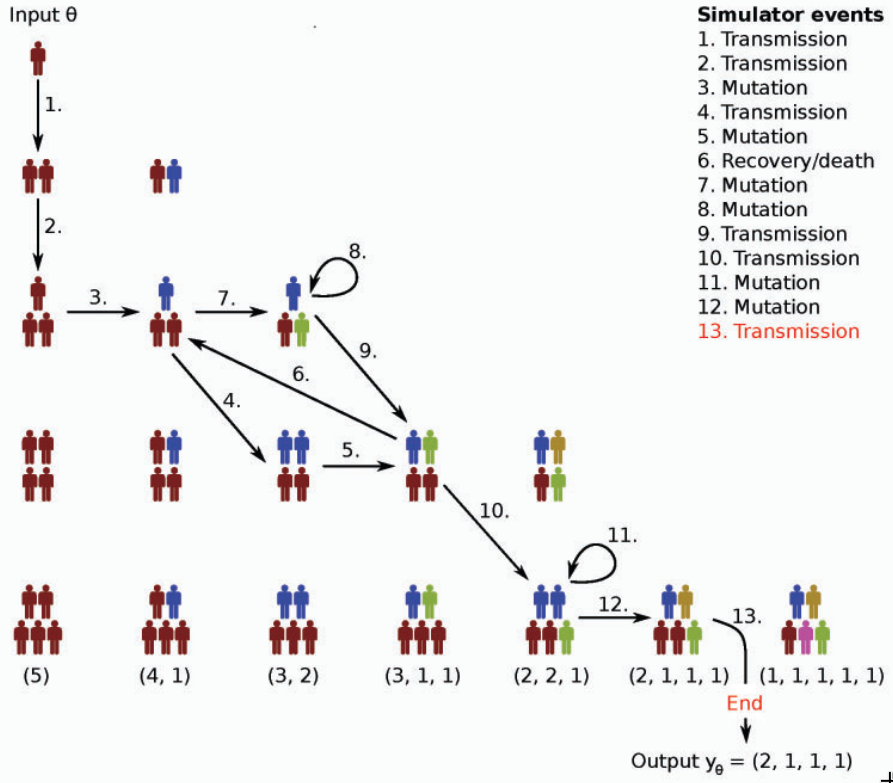
\includegraphics[width=0.75\textwidth]{./Thesis/images/chapter1/tuber_model_1.png}
    \end{center}
    \caption{Depiction of a random example from the tuberculosis
      spreading process. The image has been taken from
      \autocite{Lintusaari2017}.}
    \label{fig:tuberculosis_model}
\end{figure}

\subsubsection*{\textit{Goal of Simulation-Based Models}}

As in most Machine Learning (ML) concepts, the fundamental goal is the
derivation of one(many) parameter configuration(s) $\thetab^*$ that
\textit{describe} the data best i.e.\ generate samples
$M_r(\thetab^*)$ that are as close as possible to the observed data
$\data$. In our case, following the approach of Bayesian ML, we treat
the parameters of interest $\thetab$ as random variables and we try to
\textit{infer} a posterior distribution $p(\thetab|\data)$ on them.

\subsubsection*{\textit{Robust Optimisation Monte Carlo (ROMC) method}}

The ROMC method~\autocite{Ikonomov2019} is very a recent
likelihood-free approach. Its fundamental idea is the transformation
of the stochastic data generation process $M_r(\thetab)$ to a
deterministic mapping $g_i(\thetab)$, by sampling the variables that
produce the randomness $\vb_i \sim p(\V)$. Formally, in every
stochastic process the randomness is influenced by a vector of random
variables $\V$, whose state is unknown prior to the execution of the
simulation; sampling the state makes the procedure deterministic,
namely $g_i(\thetab) = M_d(\thetab, \V=\vb_i)$. This approach
initially introduced at \autocite{Meeds2015} with the title
\textit{Optimisation Monte Carlo (OMC)}. The ROMC extended this
approach by resolving a fundamental failure-mode of OMC\@. The ROMC
describes a methodology for approximating the posterior through a
series of steps, without explicitly enforcing which algorithms must be
utilised for each step\footnote{The implementation chooses a specific
  algorithm for each task, but this choice has just a demonstrative
  value; any appropriate algorithm can be used instead.}; in this
sense, it can be perceived as a meta-algorithm.

\subsubsection*{\textit{Implementation}}

The most important contribution of this work is the implementation of
the ROMC method in the Python package Engine for Likelihood-Free
Inference (ELFI) \autocite{1708.00707}. Since the method has been
published quite recently, it has not been implemented by now in any ML
software. This work attempts to provide the research community with a
robust and extensible implementation for further experimentation.

\subsubsection*{\textit{Explanation of simulation-based models}}

A simulator-based model is a parameterised stochastic data generating
mechanism \autocite{Gutmann2016}. The key characteristic of these
models is that although we can sample (simulate) data points, we
cannot evaluate the likelihood of a specific set of observations
$\data$. Formally, a simulator-based model is described as a
parameterised family of probability density functions
$\{ p_{\yb|\thetab}(\yb) \}_{\thetab}$, whose closed-form is either
unknown or intractable to evaluate. Whereas evaluating
$p_{\yb|\thetab}(\yb)$ is intractable, sampling is
feasible. Practically, a simulator can be understood as a black-box
machine $M_r$\footnote{The subscript $r$ in $M_r$ indicates the
  \textit{random} simulator. In the next chapters we will introduce
  $M_d$ witch stands for the \textit{deterministic} simulator.} that
given a set of parameters $\thetab$, produces samples $\yb$ in a
stochastic manner i.e.\ $M_r(\thetab) \rightarrow \yb$.

Simulator-based models are particularly captivating due to the
modelling freedom they provide; any physical process that can be
conceptualised as a computer program of finite (deterministic or
stochastic) steps can be modelled as a simulator-based model without
any compromise. The modelling freedom includes any amount of hidden
(unobserved) internal variables or logic-based decisions. As always,
this degree of freedom comes at a cost; performing the inference is
particularly demanding from both computational and mathematical
perspective. Unfortunately, the algorithms deployed so far permit the
inference only at low-dimensionality parametric spaces, i.e.\
$\thetab \in \mathbb{R}^D$ where $D$ is small.

\subsubsection*{\textit{Example}}

For underlying the importance of simulator-based models, let us use
the tuberculosis disease spread example as described in
\autocite{Tanaka2006}. An overview of the disease spread model is
presented at figure~\ref{fig:tuberculosis_model}. At each stage one of
the following \textit{unobserved} events may happen; (a) the
transmission of a specific haplotype to a new host, (b) the mutation
of an existent haplotype or (c) the exclusion of an infectious host
(recovers/dies) from the population. The random process, which stops
when $m$ infectious hosts are reached\footnote{We suppose that the
  unaffected population is infinite, so a new host can always be added
  until we reach $m$ simultaneous hosts.}, can be parameterised by the
transmission rate $\alpha$, the mutation rate $\tau$ and the exclusion
rate $\delta$, creating a $3D$-parametric space
$\thetab = (\alpha, \tau, \delta)$. The outcome of the process is a
variable-size tuple $\yb_{\thetab}$, containing the population
contaminated by each different haplotype, as described in
figure~\ref{fig:tuberculosis_model}. Let's say that the disease has
been spread in a real population and when $m$ hosts were contaminated
simultaneously, the vector with the infectious populations has been
measured to be $\data$. We would like to discover the parameters
$\thetab = (\alpha, \tau, \delta)$ that generated the spreading
process and led to the specific outcome $\data$. Computing
$p(\yb=\data|\thetab)$ requires tracking all tree-paths that could
generate the specific tuple; such exhaustive enumeration becomes
intractable when $m$ grows larger, as in real-case scenarios. In
figure~\ref{fig:tuberculosis_model} we can observe that a transmission
followed by a recovery/death creates a loop, reinstating the process
to the previous step, which also complicates the exhaustive
enumeration. Hence, representing the process with a simulator-based
model\footnote{which is simple and efficient} and performing
likelihood-free inference is the recommended solution.

\begin{figure}[!ht]
    \begin{center}
      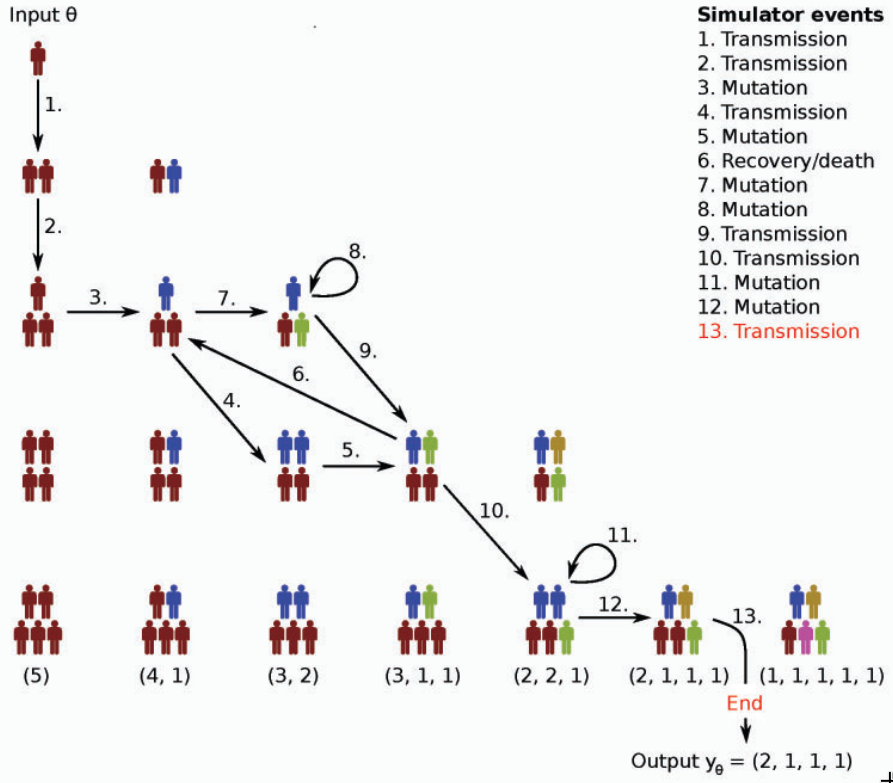
\includegraphics[width=0.75\textwidth]{./Thesis/images/chapter1/tuber_model_1.png}
    \end{center}
    \caption{Depiction of a random example from the tuberculosis
      spreading process. The image has been taken from
      \autocite{Lintusaari2017}.}
    \label{fig:tuberculosis_model}
\end{figure}

\subsubsection*{\textit{Goal of Simulation-Based Models}}

As in most Machine Learning (ML) concepts, the fundamental goal is the
derivation of one(many) parameter configuration(s) $\thetab^*$ that
\textit{describe} the data best i.e.\ generate samples
$M_r(\thetab^*)$ that are as close as possible to the observed data
$\data$. In our case, following the approach of Bayesian ML, we treat
the parameters of interest $\thetab$ as random variables and we try to
\textit{infer} a posterior distribution $p(\thetab|\data)$ on them.

\subsubsection*{\textit{Robust Optimisation Monte Carlo (ROMC) method}}

The ROMC method~\autocite{Ikonomov2019} is very a recent
likelihood-free approach. Its fundamental idea is the transformation
of the stochastic data generation process $M_r(\thetab)$ to a
deterministic mapping $g_i(\thetab)$, by sampling the variables that
produce the randomness $\vb_i \sim p(\V)$. Formally, in every
stochastic process the randomness is influenced by a vector of random
variables $\V$, whose state is unknown prior to the execution of the
simulation; sampling the state makes the procedure deterministic,
namely $g_i(\thetab) = M_d(\thetab, \V=\vb_i)$. This approach
initially introduced at \autocite{Meeds2015} with the title
\textit{Optimisation Monte Carlo (OMC)}. The ROMC extended this
approach by resolving a fundamental failure-mode of OMC\@. The ROMC
describes a methodology for approximating the posterior through a
series of steps, without explicitly enforcing which algorithms must be
utilised for each step\footnote{The implementation chooses a specific
  algorithm for each task, but this choice has just a demonstrative
  value; any appropriate algorithm can be used instead.}; in this
sense, it can be perceived as a meta-algorithm.

\subsubsection*{\textit{Implementation}}

The most important contribution of this work is the implementation of
the ROMC method in the Python package Engine for Likelihood-Free
Inference (ELFI) \autocite{1708.00707}. Since the method has been
published quite recently, it has not been implemented by now in any ML
software. This work attempts to provide the research community with a
robust and extensible implementation for further experimentation.


\subsection{Outline of Thesis}
\label{subsec:outline-of-thesis}
% The remainder of the dissertation is organized as follows. In Chapter
2 we establish the mathematical formulation; more specifically we
initially describe the Simulator-Based models and we provide some
fundamental algorithms that have been proposed for performing
statistical inference. Afterwards, we provide the mathematical
description of the ROMC approach \autocite{Ikonomov2019}. In Chapter 3, we
deal with the implementation part; we initially provide some
information regarding the Python package Engine for Likelihood-Free
Inference (ELFI) \autocite{1708.00707} and subsequently we present the
implementation details of ROMC in this package. In Chapter 4, we
illustrate the functionalities of the ROMC implementation at some
real-world examples; this chapter wishes to demonstrate the success of
the ROMC method and of our implementation at Likelihood-Free
tasks. Finally, in Chapter 5, we conclude with some thoughts on the
work we have done and some future research ideas.

The remainder of the dissertation is organized as follows. In Chapter
2 we establish the mathematical formulation; more specifically we
initially describe the Simulator-Based models and we provide some
fundamental algorithms that have been proposed for performing
statistical inference. Afterwards, we provide the mathematical
description of the ROMC approach \autocite{Ikonomov2019}. In Chapter 3, we
deal with the implementation part; we initially provide some
information regarding the Python package Engine for Likelihood-Free
Inference (ELFI) \autocite{1708.00707} and subsequently we present the
implementation details of ROMC in this package. In Chapter 4, we
illustrate the functionalities of the ROMC implementation at some
real-world examples; this chapter wishes to demonstrate the success of
the ROMC method and of our implementation at Likelihood-Free
tasks. Finally, in Chapter 5, we conclude with some thoughts on the
work we have done and some future research ideas.


\subsection{Notation}
\label{subsec:notation}
% \subsection{Notation}
\label{subsec:notation}

In this section, we keep an overview of the symbols used throughout
the document along with their explanation, in physical language. Some
quantities that are discribed informally here will be defined formally
in the next chapters. We try to keep the notation as consistent as
possible throughout the document.

 Some more generic symbols. In general, as $p(\cdot)$ we represent any valid pdf and $p(\cdot | \cdot)$ any conditional distribution. Depending on the content and the symbol used at the placeholder the distribution may have a more specific meaning.


\subsubsection*{Random Generator:}
\label{sec:random-generator}
\begin{itemize}
\item $M_r(\thetab): \R^D \rightarrow \R$
\end{itemize}

\subsubsection*{Variables}
\label{sec:variables}

\begin{itemize}
\item $D$: the dimensionality of the parameter-space
\item $\thetab \in \R^D$: the parameters of interest
\item $\data$: the observations
\item $\epsilon$: threshold
\item $\vb \in \R^N$, random variable that adds the stochasticity to the generator. 
\item $\vb_i \sim \vb$: a sample drawn from $\vb$
\item $\Y_{\thetab}$ random variable descriping the simulator $M_r(\thetab)$. The pdf of $\Y_{\thetab}$ is unknown in closed form or intractable to be evaluated.
\item $\yb_i \sim \Y_\theta$ a sample drawn from $\Y_\theta$. The sample can be obtained by executing the simulator $\yb_i \sim M_r(\thetab)$
\end{itemize}


\subsubsection*{Sets}
\label{sec:sets}

\begin{itemize}
\item $\region(\data)$ the set of points $\yb$ around the observations $\data$, i.e. $\yb := \{\yb: d(\yb, \data) < \epsilon \}$
\item $\regioni = \region(\yb_i)$ the set of points $\yb$ around $\yb_i$, i.e. $\yb := \{\yb: d(\yb, \yb_i) < \epsilon \}$
\end{itemize}
    
\subsubsection*{Generic Functions}
\label{sec:generic-functions}

\begin{itemize}
\item $p(\thetab)$: the prior distribution
\item $p(\thetab|\data)$: the posterior distribution
\item $p_{d,\epsilon}(\thetab|\data)$: the approximate posterior distribution
\item $d(\mathbf{x}, \mathbf{y}): \R^{2N} \rightarrow \R$: any valid distance, e.g L2 norm: $||\mathbf{x}-\mathbf{y}||_2^2$
\end{itemize}

\subsubsection*{Functions (Mappings):}
\label{sec:functions-mappings}

\begin{itemize}
\item $M_d(\thetab, \vb): \R^D \rightarrow \R$ the deterministic generator; if we pass the state $v$ of all stochastic variables that are part of the data generation process, then producing an outcome becomes deterministic.
\item $f_i(\thetab) = M_d(\thetab, \vb_i)$ alias

\item $g_i(\thetab) = d(f_i(\thetab), \data)$
\item $T(\mathbf{x}): \mathbb{R}^{D_1} \rightarrow \mathbb{R}^{D_2}$ where $D_1 > D_2$, the summary statistic mapping.
\item  $\indicator{\region(\data)}(\yb)$ the indicator function:
    \begin{gather*}\indicator{\region(\data)}(\yb) = \left\{
	\begin{array}{ll}
		1 & \mbox{if } d(\yb,\data) \leq \epsilon \\
		0 & \mbox{else } 
	\end{array} \right. \end{gather*}

\item $L(\theta)$ the likelihood function
\item $L_{d,\epsilon}(\theta)$ the approximate likelihood function
\end{itemize}   

\subsection{Notation}
\label{subsec:notation}

In this section, we keep an overview of the symbols used throughout
the document along with their explanation, in physical language. Some
quantities that are discribed informally here will be defined formally
in the next chapters. We try to keep the notation as consistent as
possible throughout the document.

 Some more generic symbols. In general, as $p(\cdot)$ we represent any valid pdf and $p(\cdot | \cdot)$ any conditional distribution. Depending on the content and the symbol used at the placeholder the distribution may have a more specific meaning.


\subsubsection*{Random Generator:}
\label{sec:random-generator}
\begin{itemize}
\item $M_r(\thetab): \R^D \rightarrow \R$
\end{itemize}

\subsubsection*{Variables}
\label{sec:variables}

\begin{itemize}
\item $D$: the dimensionality of the parameter-space
\item $\thetab \in \R^D$: the parameters of interest
\item $\data$: the observations
\item $\epsilon$: threshold
\item $\vb \in \R^N$, random variable that adds the stochasticity to the generator. 
\item $\vb_i \sim \vb$: a sample drawn from $\vb$
\item $\Y_{\thetab}$ random variable descriping the simulator $M_r(\thetab)$. The pdf of $\Y_{\thetab}$ is unknown in closed form or intractable to be evaluated.
\item $\yb_i \sim \Y_\theta$ a sample drawn from $\Y_\theta$. The sample can be obtained by executing the simulator $\yb_i \sim M_r(\thetab)$
\end{itemize}


\subsubsection*{Sets}
\label{sec:sets}

\begin{itemize}
\item $\region(\data)$ the set of points $\yb$ around the observations $\data$, i.e. $\yb := \{\yb: d(\yb, \data) < \epsilon \}$
\item $\regioni = \region(\yb_i)$ the set of points $\yb$ around $\yb_i$, i.e. $\yb := \{\yb: d(\yb, \yb_i) < \epsilon \}$
\end{itemize}
    
\subsubsection*{Generic Functions}
\label{sec:generic-functions}

\begin{itemize}
\item $p(\thetab)$: the prior distribution
\item $p(\thetab|\data)$: the posterior distribution
\item $p_{d,\epsilon}(\thetab|\data)$: the approximate posterior distribution
\item $d(\mathbf{x}, \mathbf{y}): \R^{2N} \rightarrow \R$: any valid distance, e.g L2 norm: $||\mathbf{x}-\mathbf{y}||_2^2$
\end{itemize}

\subsubsection*{Functions (Mappings):}
\label{sec:functions-mappings}

\begin{itemize}
\item $M_d(\thetab, \vb): \R^D \rightarrow \R$ the deterministic generator; if we pass the state $v$ of all stochastic variables that are part of the data generation process, then producing an outcome becomes deterministic.
\item $f_i(\thetab) = M_d(\thetab, \vb_i)$ alias

\item $g_i(\thetab) = d(f_i(\thetab), \data)$
\item $T(\mathbf{x}): \mathbb{R}^{D_1} \rightarrow \mathbb{R}^{D_2}$ where $D_1 > D_2$, the summary statistic mapping.
\item  $\indicator{\region(\data)}(\yb)$ the indicator function:
    \begin{gather*}\indicator{\region(\data)}(\yb) = \left\{
	\begin{array}{ll}
		1 & \mbox{if } d(\yb,\data) \leq \epsilon \\
		0 & \mbox{else } 
	\end{array} \right. \end{gather*}

\item $L(\theta)$ the likelihood function
\item $L_{d,\epsilon}(\theta)$ the approximate likelihood function
\end{itemize}   


%%%%%%%%%%%%%%%%%%%%%%%%%%%%%%%%%%%%%%%%
\clearpage
\section{Background}
\label{sec:background}

\subsection{Simulator-based models}
% As already stated at Chapter~\ref{sec:introduction}, in
simulator-based models we cannot evaluate the posterior
$p(\thetab|\data) \propto L(\thetab)p(\thetab)$, due to the
intractability of the likelihood $L(\thetab) = p(\data|\thetab)$. The
following equation allows incorporating the simulator in the place of
the likelihood and forms the basis of all likelihood-free inference
approaches,

\begin{equation} \label{eq:likelihood}
  L(\thetab) =
  \lim_{\epsilon \to 0} c_\epsilon \int_{\yb \in B_{d,\epsilon}(\data)} p(\yb|\thetab)d\yb =
  \lim_{\epsilon \to 0} c_\epsilon \Pr(M_r(\thetab) \in B_{d,\epsilon}(\data))
\end{equation}
%
where $c_\epsilon$ is a proportionality factor dependent on
$\epsilon$, needed when
$\Pr(M_r(\thetab) \in B_{d, \epsilon}(\data)) \rightarrow 0$, as
$\epsilon \rightarrow 0$. Equation~\ref{eq:likelihood} describes that
the likelihood of a specific parameter configuration $\thetab$ is
proportional to the probability that the simulator will produce
outputs equal to the observations, using this configuration.

\subsubsection{Approximate Bayesian Computation (ABC) Rejection
  Sampling}

ABC rejection sampling is a modified version of the traditional
rejection sampling method, for cases when the evaluation of the
likelihood is intractable. In the typical rejection sampling, a sample
obtained from the prior $\thetab \sim p(\thetab)$ gets accepted
with probability $L(\thetab)/ \text{max}_{\thetab}
L(\thetab)$. Though we cannot use this approach out-of-the-box
(evaluating $L(\thetab)$ is impossible in our case), we can
modify the method incorporating the simulator.

In the discrete case scenario where $\Y_{\thetab}$ can take a finite
set of values, the likelihood becomes
$L(\thetab) = \Pr(\Y_{\thetab} = \data)$ and the posterior
$p(\thetab|\data) \propto \Pr(\Y_{\thetab}=\data)p(\thetab)$; hence, we can
sample from the prior $\thetab_i \sim p(\thetab)$, run the simulator
$\yb_i = M_r(\thetab_i)$ and accept $\thetab_i$ only if
$\yb_i = \data$.

The method above becomes less useful as the finite set of
$\Y_{\thetab}$ values grows larger, since the probability of
accepting a sample becomes smaller. In the limit
where the set becomes infinite (i.e.\ continuous case) the probability
becomes zero. In order for the method to work in this set-up, a
relaxation is introduced; we relax the acceptance criterion by letting
$\yb_{i}$ lie in a larger set of points i.e.\
$\yb_{i} \in \region(\data), \epsilon > 0$. The region can be
defined as $\region (\data) := \{\yb: d(\yb, \data) \leq \epsilon \}$
where $d(\cdot, \cdot)$ can represent any valid distance. With this
modification, the maintained samples follow the approximate posterior,

\begin{equation} \label{eq:approx_posterior}
  p_{d,\epsilon}(\thetab|\data) \propto Pr(\yb \in
  \region(\data)) p(\thetab)
\end{equation}

\noindent
This method is called Rejection ABC.

\subsubsection{Summary Statistics}

When $\yb \in \mathbb{R}^D$ lies in a high-dimensional space, generating
samples inside $\region (\data)$ becomes rare even when $\epsilon$ is
relatively large; this is the curse of dimensionality. As a
representative example lets make the following hypothesis;

\begin{itemize}
\item $d$ is set to be the Euclidean distance, hence
  $\region(\data) := \{ \yb: ||\yb - \data||_2^2 < \epsilon^2 \}$ is a
  hyper-sphere with radius $\epsilon$ and volume $V_{hypersphere} = \frac{\pi^{D/2}}{\Gamma(D/2 + 1)} \epsilon^D$
\item the prior $p(\thetab)$ is a uniform distribution in a hyper-cube with side of
  length $2\epsilon$ and volume $V_{hypercube} = (2\epsilon)^D$
\item the generative model is the identity function $\yb=f(\thetab)= \thetab $
\end{itemize}

\noindent
The probability of drawing a sample inside the hypersphere equals the
fraction of the volume of the hypersphere inscribed in the hypercube:

\begin{equation}
  Pr(\yb \in \region (\data))
  = Pr(\thetab \in \region (\data))
  = \frac{V_{hypersphere}}{V_{hypercube}}
  = \frac{\pi^{D/2}}{2^D\Gamma(D/2 + 1)} \rightarrow 0, \quad \text{as} \quad D \rightarrow \infty
\end{equation}

\noindent
We observe that the probability tends to $0$, independently of
$\epsilon$; enlarging $\epsilon$ will not increase the acceptance
rate. Intuitively, we can think that in high-dimensional spaces the
volume of the hypercube concentrates at its corners. This generates
the need for a mapping
$T: \mathbb{R}^{D_1} \rightarrow \mathbb{R}^{D_2}$ where $D_1 > D_2$,
for squeezing the dimensionality of the output. This
dimensionality-reduction step that redefines the area as
$\region(\data) := \{\yb: d(T(\yb), T(\data)) \leq \epsilon \}$ is
called \textit{summary statistic} extraction, since the distance is
not measured on the actual outputs, but on a summarisation (i.e.\
lower-dimension representation) of them.

\subsubsection{Approximations introduced so far}

So far, we have introduced some approximations for inferring the
posterior as
$p_{d,\epsilon}(\thetab|\data) \propto Pr(\Y_{\thetab} \in
\region(\data))p(\thetab)$ where
$\region(\data) := \{\yb: d(T(\yb), T(\data)) < \epsilon \}$. These
approximations introduce two different types of errors:

\begin{itemize}
\item $\epsilon$ is chosen to be \textit{big enough}, so that enough
  samples are accepted. This modification leads to the approximate
  posterior introduced in \eqref{eq:approx_posterior}
\item $T$ introduces some loss of information, making possible a $\yb$
  far away from $\data$ i.e.\ $\yb: d(\yb,\data)>\epsilon$, to enter
  the acceptance region after the dimensionality reduction
  $d(T(\yb), T(\data)) \leq \epsilon$
\end{itemize}

\noindent
In the following sections, we will not use the summary statistics in
our expressions for the notation not to clutter. One could understand
it as absorbing the mapping $T(\cdot)$ inside the simulator. In any
case, all the propositions that will be expressed in the following
sections are valid with the use of summary statistics.
  
\subsubsection{Optimisation Monte Carlo (OMC)}

Before we define the likelihood approximation as introduced in the
OMC, approach lets define the indicator function based on
$\region(\yb)$. The indicator function $\indicator{\region(\yb)}(\xb)$
returns 1 if $\xb \in \region(\yb)$ and 0 otherwise. If
$d(\cdot,\cdot)$ is a formal distance, due to symmetry
$\indicator{\region(\yb)}(\xb) = \indicator{\region(\xb)}(\yb)$, so
the expressions can be used interchangeably.

\begin{gather} \label{eq:indicator} \indicator{\region(\yb)}(\xb)=
  \left\{
    \begin{array}{ll}
      1 & \mbox{if } \xb \in \region(\yb) \\
      0 & \mbox{otherwise} 
    \end{array} \right. \end{gather}

\noindent
Based on equation~\eqref{eq:approx_posterior} and the indicator
function as defined above~\eqref{eq:indicator}, we can approximate the
likelihood as:

\begin{gather} \label{eq:approx_likelihood}
  L_{d, \epsilon}(\thetab) =
  \int_{\yb \in B_\epsilon(\data)}p(\yb|\thetab)d\yb =
  \int_{\yb \in \R^D} \indicator{\region(\data)}(\yb)p(\yb|\thetab)d\yb\\
  \approx \frac{1}{N} \sum_i^N \indicator{\region(\data)}(\yb_i),\text{ where }
  \yb_i \sim M_r(\thetab) \label{eq:init_view}\\
  \approx \frac{1}{N} \sum_i^N \indicator{\region (\data)} (\yb_i)
  \text{ where } \yb_i = M_d(\thetab, \vb_i), \vb_i \sim p(\vb) \label{eq:alt_view}
\end{gather}
%
This approach is quite intuitive; approximating the likelihood of a
specific $\thetab$ requires sampling from the data generator and count
the fraction of samples that lie inside the area around the
observations. Nevertheless, by using the approximation of equation
\eqref{eq:init_view} we need to draw $N$ new samples for each distinct
evaluation of $L_{d,\epsilon}(\thetab)$; this makes this approach
quite inconvenient from a computational point-of-view. For this
reason, we choose to approximate the integral as in equation
\eqref{eq:alt_view}; the nuisance variables are sampled once
$\vb_i \sim p(\vb)$ and we count the fraction of samples that lie
inside the area using the deterministic simulators
$M_d(\thetab, \vb_i) \: \forall i$. Hence, the evaluation
$L_{d,\epsilon}(\thetab)$ for each different $\thetab$ does not imply
drawing new samples all over again. Based on this approach, the
unnormalised approximate posterior can be defined as:

\begin{equation} \label{eq:aprox_posterior}
  p_{d,\epsilon}(\thetab|\data)
  \propto p(\thetab) \sum_i^N \indicator{ \region(\data)} (\yb_i)
\end{equation}

\subsubsection*{Further approximations for sampling and computing expectations}

The posterior approximation in \eqref{eq:approx_posterior} does not
provide any obvious way for drawing samples. In fact, the set
$\mathcal{S}_i = \{ \thetab: M_d(\thetab, \vb_i) \in \region(\data) \}$ can
represent any arbitrary shape in the D-dimensional Euclidean space; it
can be non-convex, can contain disjoint sets of $\thetab$ etc. We need
some further simplification of the posterior for being able to draw
samples from it.

As a side-note, weighted sampling could be performed in a
straightforward fashion with importance sampling. Using the prior as
the proposal distribution $\thetab_i \sim p(\thetab)$ and we can
compute the weight as
$w_i = \frac{L_{d,\epsilon}(\thetab_i)}{p(\thetab_i)}$, where
$L_{d,\epsilon}(\thetab_i)$ is computed with the expression
\eqref{eq:approx_likelihood}. This approach has the same drawbacks as
ABC rejection sampling; when the prior is wide or the dimensionality
$D$ is high, drawing a sample with non-zero weight is rare, leading to
either poor Effective Sample Size (ESS) or huge execution time.

The OMC proposes a quite drastic simplification of the posterior; it
squeezes all regions $\mathcal{S}_i$ into a single point
$\thetab_i^* \in \mathcal{S}_i$ attaching a weight $w_i$ proportional
to the volume of $\mathcal{S}_i$. For obtaining a
$\thetab_i^* \in \mathcal{S}_i$, a gradient based optimiser is used
for minimising $g_i(\thetab) = d(\data, f_i(\thetab))$ and the
estimation of the volume of $\mathcal{S}_i$ is done using the Hessian
approximation $\hess_i \approx \jac_i^{*T}\jac_i^*$, where $\jac_i^*$
is the Jacobian matrix of $g_i(\thetab)$ at $\thetab_i^*$. Hence,

\begin{gather} \label{eq:OMC_posterior}
    p(\thetab|\data) \propto p(\thetab) \sum_i^N w_i \delta(\thetab - \thetab_i^*)\\
  \thetab_i^* = \text{argmin}_{\thetab} \:g_i(\thetab) \\
  w_i \propto \frac{1}{\sqrt{det( \jac_i^{*T}\jac_i^*)}}
\end{gather}

The distribution \eqref{eq:OMC_posterior} provides weighted samples
automatically and an expectation can be computed easily with the
following equation,

\begin{equation}
  \label{eq:OMC_expectation}
  E_{p(\thetab|\data)}[h(\thetab)] = \frac{\sum_i^N w_i p(\thetab_i^*)h(\thetab_i^*)}{\sum_i^N w_i p(\thetab_i^*)}
\end{equation}

As already stated at Chapter~\ref{sec:introduction}, in
simulator-based models we cannot evaluate the posterior
$p(\thetab|\data) \propto L(\thetab)p(\thetab)$, due to the
intractability of the likelihood $L(\thetab) = p(\data|\thetab)$. The
following equation allows incorporating the simulator in the place of
the likelihood and forms the basis of all likelihood-free inference
approaches,

\begin{equation} \label{eq:likelihood}
  L(\thetab) =
  \lim_{\epsilon \to 0} c_\epsilon \int_{\yb \in B_{d,\epsilon}(\data)} p(\yb|\thetab)d\yb =
  \lim_{\epsilon \to 0} c_\epsilon \Pr(M_r(\thetab) \in B_{d,\epsilon}(\data))
\end{equation}
%
where $c_\epsilon$ is a proportionality factor dependent on
$\epsilon$, needed when
$\Pr(M_r(\thetab) \in B_{d, \epsilon}(\data)) \rightarrow 0$, as
$\epsilon \rightarrow 0$. Equation~\ref{eq:likelihood} describes that
the likelihood of a specific parameter configuration $\thetab$ is
proportional to the probability that the simulator will produce
outputs equal to the observations, using this configuration.

\subsubsection{Approximate Bayesian Computation (ABC) Rejection
  Sampling}

ABC rejection sampling is a modified version of the traditional
rejection sampling method, for cases when the evaluation of the
likelihood is intractable. In the typical rejection sampling, a sample
obtained from the prior $\thetab \sim p(\thetab)$ gets accepted
with probability $L(\thetab)/ \text{max}_{\thetab}
L(\thetab)$. Though we cannot use this approach out-of-the-box
(evaluating $L(\thetab)$ is impossible in our case), we can
modify the method incorporating the simulator.

In the discrete case scenario where $\Y_{\thetab}$ can take a finite
set of values, the likelihood becomes
$L(\thetab) = \Pr(\Y_{\thetab} = \data)$ and the posterior
$p(\thetab|\data) \propto \Pr(\Y_{\thetab}=\data)p(\thetab)$; hence, we can
sample from the prior $\thetab_i \sim p(\thetab)$, run the simulator
$\yb_i = M_r(\thetab_i)$ and accept $\thetab_i$ only if
$\yb_i = \data$.

The method above becomes less useful as the finite set of
$\Y_{\thetab}$ values grows larger, since the probability of
accepting a sample becomes smaller. In the limit
where the set becomes infinite (i.e.\ continuous case) the probability
becomes zero. In order for the method to work in this set-up, a
relaxation is introduced; we relax the acceptance criterion by letting
$\yb_{i}$ lie in a larger set of points i.e.\
$\yb_{i} \in \region(\data), \epsilon > 0$. The region can be
defined as $\region (\data) := \{\yb: d(\yb, \data) \leq \epsilon \}$
where $d(\cdot, \cdot)$ can represent any valid distance. With this
modification, the maintained samples follow the approximate posterior,

\begin{equation} \label{eq:approx_posterior}
  p_{d,\epsilon}(\thetab|\data) \propto Pr(\yb \in
  \region(\data)) p(\thetab)
\end{equation}

\noindent
This method is called Rejection ABC.

\subsubsection{Summary Statistics}

When $\yb \in \mathbb{R}^D$ lies in a high-dimensional space, generating
samples inside $\region (\data)$ becomes rare even when $\epsilon$ is
relatively large; this is the curse of dimensionality. As a
representative example lets make the following hypothesis;

\begin{itemize}
\item $d$ is set to be the Euclidean distance, hence
  $\region(\data) := \{ \yb: ||\yb - \data||_2^2 < \epsilon^2 \}$ is a
  hyper-sphere with radius $\epsilon$ and volume $V_{hypersphere} = \frac{\pi^{D/2}}{\Gamma(D/2 + 1)} \epsilon^D$
\item the prior $p(\thetab)$ is a uniform distribution in a hyper-cube with side of
  length $2\epsilon$ and volume $V_{hypercube} = (2\epsilon)^D$
\item the generative model is the identity function $\yb=f(\thetab)= \thetab $
\end{itemize}

\noindent
The probability of drawing a sample inside the hypersphere equals the
fraction of the volume of the hypersphere inscribed in the hypercube:

\begin{equation}
  Pr(\yb \in \region (\data))
  = Pr(\thetab \in \region (\data))
  = \frac{V_{hypersphere}}{V_{hypercube}}
  = \frac{\pi^{D/2}}{2^D\Gamma(D/2 + 1)} \rightarrow 0, \quad \text{as} \quad D \rightarrow \infty
\end{equation}

\noindent
We observe that the probability tends to $0$, independently of
$\epsilon$; enlarging $\epsilon$ will not increase the acceptance
rate. Intuitively, we can think that in high-dimensional spaces the
volume of the hypercube concentrates at its corners. This generates
the need for a mapping
$T: \mathbb{R}^{D_1} \rightarrow \mathbb{R}^{D_2}$ where $D_1 > D_2$,
for squeezing the dimensionality of the output. This
dimensionality-reduction step that redefines the area as
$\region(\data) := \{\yb: d(T(\yb), T(\data)) \leq \epsilon \}$ is
called \textit{summary statistic} extraction, since the distance is
not measured on the actual outputs, but on a summarisation (i.e.\
lower-dimension representation) of them.

\subsubsection{Approximations introduced so far}

So far, we have introduced some approximations for inferring the
posterior as
$p_{d,\epsilon}(\thetab|\data) \propto Pr(\Y_{\thetab} \in
\region(\data))p(\thetab)$ where
$\region(\data) := \{\yb: d(T(\yb), T(\data)) < \epsilon \}$. These
approximations introduce two different types of errors:

\begin{itemize}
\item $\epsilon$ is chosen to be \textit{big enough}, so that enough
  samples are accepted. This modification leads to the approximate
  posterior introduced in \eqref{eq:approx_posterior}
\item $T$ introduces some loss of information, making possible a $\yb$
  far away from $\data$ i.e.\ $\yb: d(\yb,\data)>\epsilon$, to enter
  the acceptance region after the dimensionality reduction
  $d(T(\yb), T(\data)) \leq \epsilon$
\end{itemize}

\noindent
In the following sections, we will not use the summary statistics in
our expressions for the notation not to clutter. One could understand
it as absorbing the mapping $T(\cdot)$ inside the simulator. In any
case, all the propositions that will be expressed in the following
sections are valid with the use of summary statistics.
  
\subsubsection{Optimisation Monte Carlo (OMC)}

Before we define the likelihood approximation as introduced in the
OMC, approach lets define the indicator function based on
$\region(\yb)$. The indicator function $\indicator{\region(\yb)}(\xb)$
returns 1 if $\xb \in \region(\yb)$ and 0 otherwise. If
$d(\cdot,\cdot)$ is a formal distance, due to symmetry
$\indicator{\region(\yb)}(\xb) = \indicator{\region(\xb)}(\yb)$, so
the expressions can be used interchangeably.

\begin{gather} \label{eq:indicator} \indicator{\region(\yb)}(\xb)=
  \left\{
    \begin{array}{ll}
      1 & \mbox{if } \xb \in \region(\yb) \\
      0 & \mbox{otherwise} 
    \end{array} \right. \end{gather}

\noindent
Based on equation~\eqref{eq:approx_posterior} and the indicator
function as defined above~\eqref{eq:indicator}, we can approximate the
likelihood as:

\begin{gather} \label{eq:approx_likelihood}
  L_{d, \epsilon}(\thetab) =
  \int_{\yb \in B_\epsilon(\data)}p(\yb|\thetab)d\yb =
  \int_{\yb \in \R^D} \indicator{\region(\data)}(\yb)p(\yb|\thetab)d\yb\\
  \approx \frac{1}{N} \sum_i^N \indicator{\region(\data)}(\yb_i),\text{ where }
  \yb_i \sim M_r(\thetab) \label{eq:init_view}\\
  \approx \frac{1}{N} \sum_i^N \indicator{\region (\data)} (\yb_i)
  \text{ where } \yb_i = M_d(\thetab, \vb_i), \vb_i \sim p(\vb) \label{eq:alt_view}
\end{gather}
%
This approach is quite intuitive; approximating the likelihood of a
specific $\thetab$ requires sampling from the data generator and count
the fraction of samples that lie inside the area around the
observations. Nevertheless, by using the approximation of equation
\eqref{eq:init_view} we need to draw $N$ new samples for each distinct
evaluation of $L_{d,\epsilon}(\thetab)$; this makes this approach
quite inconvenient from a computational point-of-view. For this
reason, we choose to approximate the integral as in equation
\eqref{eq:alt_view}; the nuisance variables are sampled once
$\vb_i \sim p(\vb)$ and we count the fraction of samples that lie
inside the area using the deterministic simulators
$M_d(\thetab, \vb_i) \: \forall i$. Hence, the evaluation
$L_{d,\epsilon}(\thetab)$ for each different $\thetab$ does not imply
drawing new samples all over again. Based on this approach, the
unnormalised approximate posterior can be defined as:

\begin{equation} \label{eq:aprox_posterior}
  p_{d,\epsilon}(\thetab|\data)
  \propto p(\thetab) \sum_i^N \indicator{ \region(\data)} (\yb_i)
\end{equation}

\subsubsection*{Further approximations for sampling and computing expectations}

The posterior approximation in \eqref{eq:approx_posterior} does not
provide any obvious way for drawing samples. In fact, the set
$\mathcal{S}_i = \{ \thetab: M_d(\thetab, \vb_i) \in \region(\data) \}$ can
represent any arbitrary shape in the D-dimensional Euclidean space; it
can be non-convex, can contain disjoint sets of $\thetab$ etc. We need
some further simplification of the posterior for being able to draw
samples from it.

As a side-note, weighted sampling could be performed in a
straightforward fashion with importance sampling. Using the prior as
the proposal distribution $\thetab_i \sim p(\thetab)$ and we can
compute the weight as
$w_i = \frac{L_{d,\epsilon}(\thetab_i)}{p(\thetab_i)}$, where
$L_{d,\epsilon}(\thetab_i)$ is computed with the expression
\eqref{eq:approx_likelihood}. This approach has the same drawbacks as
ABC rejection sampling; when the prior is wide or the dimensionality
$D$ is high, drawing a sample with non-zero weight is rare, leading to
either poor Effective Sample Size (ESS) or huge execution time.

The OMC proposes a quite drastic simplification of the posterior; it
squeezes all regions $\mathcal{S}_i$ into a single point
$\thetab_i^* \in \mathcal{S}_i$ attaching a weight $w_i$ proportional
to the volume of $\mathcal{S}_i$. For obtaining a
$\thetab_i^* \in \mathcal{S}_i$, a gradient based optimiser is used
for minimising $g_i(\thetab) = d(\data, f_i(\thetab))$ and the
estimation of the volume of $\mathcal{S}_i$ is done using the Hessian
approximation $\hess_i \approx \jac_i^{*T}\jac_i^*$, where $\jac_i^*$
is the Jacobian matrix of $g_i(\thetab)$ at $\thetab_i^*$. Hence,

\begin{gather} \label{eq:OMC_posterior}
    p(\thetab|\data) \propto p(\thetab) \sum_i^N w_i \delta(\thetab - \thetab_i^*)\\
  \thetab_i^* = \text{argmin}_{\thetab} \:g_i(\thetab) \\
  w_i \propto \frac{1}{\sqrt{det( \jac_i^{*T}\jac_i^*)}}
\end{gather}

The distribution \eqref{eq:OMC_posterior} provides weighted samples
automatically and an expectation can be computed easily with the
following equation,

\begin{equation}
  \label{eq:OMC_expectation}
  E_{p(\thetab|\data)}[h(\thetab)] = \frac{\sum_i^N w_i p(\thetab_i^*)h(\thetab_i^*)}{\sum_i^N w_i p(\thetab_i^*)}
\end{equation}


\subsection{Robust Optimisation Monte Carlo (ROMC) approach}
\label{sec:ROMC}
% The simplifications introduced by OMC, although quite useful from a
computational point-of-view, they suffer from some significant failure modes:

\begin{itemize}
\item The whole acceptable region $S_i$, for each nuisance variable,
  shrinks to a single point $\thetab_i^*$; this simplification may add
  significant error when then the area $S_i$ is relatively big.
\item The weight $w_i$ is computed using information from $\thetab_i^*$, i.e.\ the curvature of $g_i$ at the point
  $\thetab_i^*$. This approach can introduce significant error when
  $g_i$ is almost flat at $\thetab_i^*$, leading to a
  $\text{det}(\jac_i^{*T}\jac_i^*) \rightarrow 0 \Rightarrow w_i
  \rightarrow \infty$, thus dominating the posterior.
\item There is no way to solve the optimisation problem
  $\thetab_i^* = \text{argmin}_{\thetab} \: [g_i(\thetab)]$ when $g_i$
  is not differentiable.
\end{itemize}


\subsubsection{Sampling and computing expectation in ROMC}

The ROMC approach resolves the aforementioned issues. Instead of
collapsing the acceptance regions into single points, it tries to
approximate them with a bounding box and then defines a uniform
distribution over it.\footnote{The description on how to estimate the
  bounding box is provided in the following chapters.}, which serves as the proposal distribution for importance sampling. If we
define as $q_i$, the uniform distribution defined on the $i-th$
bounding box, weighted sampling is performed as:

\begin{gather}
  \label{eq:sampling}
  \thetab_{ij} \sim q_i \\
  w_{ij} = \frac{\indicator{\region(\data)}(M_d(\thetab_{ij}, \vb_i)) p(\thetab_{ij})}{q(\thetab_{ij})}
\end{gather}

\noindent
Having defined the procedure for obtaining weighted samples, any expectation $E_{p(\thetab|\data)}[h(\thetab)]$, can be approximated as,

\begin{equation} \label{eq:expectation}
  E_{p(\thetab|\data)}[h(\thetab)] \approx \frac{\sum_{ij} w_{ij} h(\thetab_{ij})}{\sum_{ij} w_{ij}}
\end{equation}


\subsubsection{Construction of the proposal region}

In this section we will describe mathematically the steps needed for
computing the proposal distributions $q_i$. There will be also
presented a Bayesian optimisation alternative when gradients are not
available.

\subsubsection*{Define and solve deterministic optimisation problems}

For each set of nuisance variables $\vb_i, i = \{1,2,...,n_1 \}$ a
deterministic function is defined as
$f_i(\thetab) = M_d(\thetab,\vb_i)$. For constructing the proposal
region, we search for a point
$\thetab_* : d(f_i(\thetab_*), \data) < \epsilon$; this point can be
obtained by solving the the following optimisation problem:

\begin{subequations}
\begin{alignat}{2}
&\!\min_{\thetab}        &\qquad& g_i(\thetab) = d(\data,  f_i(\thetab))\label{eq:optProb}\\
&\text{subject to} &      & g_i(\thetab) \leq \epsilon
\end{alignat}
\end{subequations}
%
We maintain a list of the solutions $\thetab_i^*$ of the optimisation
problems. If for a specific set of nuisance variables $\vb_i$, there
is no feasible solution we add nothing to the list. The optimisation
problem can be treated as unconstrained, accepting the optimal point
$\thetab_i^* = \text{argmin}_{\thetab} g_i(\thetab)$ only if
$g_i(\thetab_i^*) < \epsilon$.

\subsubsection*{Gradient-based approach}
\label{subsubsec:GB_approach}

The nature of the generative model $M_r(\thetab)$, specifies the
properties of the objective function $g_i$. If $g_i$ is continuous
with smooth gradients $\nabla_{\thetab} g_i$ any gradient-based
iterative algorithm can be used for solving~\ref{eq:optProb}. The
gradients $\nabla_{\thetab} g_i$ can be either provided in closed form
or be approximated by finite differences.

\subsubsection*{Bayesian optimisation approach}
\label{subsubsec:GP_approach}

In cases where the gradients are not available, the Bayesian
optimisation scheme provides an alternative
choice~\autocite{Shahriari2016}. With this approach, apart from
obtaining an optimal $\thetab_i^* $, a surrogate model $\hat{d}_i$ of
the distance $g_i$ is fitted; this approximate model can be used in
the following steps for making the method more
efficient. Specifically, in the construction of the proposal region
and in
equations~\eqref{eq:approx_posterior},~\eqref{eq:sampling},~\eqref{eq:expectation}
it could replace $g_i$ in the evaluation of the indicator
function, providing a major speed-up.

\subsubsection*{Construction of the proposal area $q_i$}

After obtaining a $\thetab_i^*$ such that $g_i(\thetab_i^*) < \epsilon$,
we need to construct a bounding box around it. The bounding box must
contain the acceptance region around $\thetab_i^*$, i.e.\
$\{ \thetab : g_i(\thetab) < \epsilon$ and
$d(\thetab, \thetab_i^*) < M \}$. The second condition
$d(\thetab, \thetab_i^*) < M$ is meant to describe that if
$S_i := \{ \thetab : g_i(\thetab) < \epsilon \} $ contains a number of
disjoint sets of $\thetab$ that respect $g_i(\thetab) < \epsilon$, we
want our bounding box to fit only the one that contains $\thetab_i^*$. We
seek for a bounding box that is as tight as possible to the local
acceptance region (enlarging the bounding box without a reason decreases the acceptance
rate) but large enough for not discarding accepted areas. 

In contrast with the OMC approach, we construct the bounding box by
obtaining search directions and querying the indicator function as we move on them. The
search directions $\mathbf{v}_d$ are computed as the eigenvectors of
the curvature at $\thetab_i^*$ and a line-search method is used to
obtain the limit point where
$g_i(\thetab_i^* + \kappa \vb_d) \geq
\epsilon$\footnote{$-\kappa$ is used as well for the opposite direction along the search line}. The Algorithm~\ref{alg:region_construction} describes the method in-depth. After the limits are obtained along all
search directions, we define bounding box and the uniform distribution $q_i$. This is the proposal distribution used for the importance
sampling as explained in \eqref{eq:sampling}.

The simplifications introduced by OMC, although quite useful from a
computational point-of-view, they suffer from some significant failure modes:

\begin{itemize}
\item The whole acceptable region $S_i$, for each nuisance variable,
  shrinks to a single point $\thetab_i^*$; this simplification may add
  significant error when then the area $S_i$ is relatively big.
\item The weight $w_i$ is computed using information from $\thetab_i^*$, i.e.\ the curvature of $g_i$ at the point
  $\thetab_i^*$. This approach can introduce significant error when
  $g_i$ is almost flat at $\thetab_i^*$, leading to a
  $\text{det}(\jac_i^{*T}\jac_i^*) \rightarrow 0 \Rightarrow w_i
  \rightarrow \infty$, thus dominating the posterior.
\item There is no way to solve the optimisation problem
  $\thetab_i^* = \text{argmin}_{\thetab} \: [g_i(\thetab)]$ when $g_i$
  is not differentiable.
\end{itemize}


\subsubsection{Sampling and computing expectation in ROMC}

The ROMC approach resolves the aforementioned issues. Instead of
collapsing the acceptance regions into single points, it tries to
approximate them with a bounding box and then defines a uniform
distribution over it.\footnote{The description on how to estimate the
  bounding box is provided in the following chapters.}, which serves as the proposal distribution for importance sampling. If we
define as $q_i$, the uniform distribution defined on the $i-th$
bounding box, weighted sampling is performed as:

\begin{gather}
  \label{eq:sampling}
  \thetab_{ij} \sim q_i \\
  w_{ij} = \frac{\indicator{\region(\data)}(M_d(\thetab_{ij}, \vb_i)) p(\thetab_{ij})}{q(\thetab_{ij})}
\end{gather}

\noindent
Having defined the procedure for obtaining weighted samples, any expectation $E_{p(\thetab|\data)}[h(\thetab)]$, can be approximated as,

\begin{equation} \label{eq:expectation}
  E_{p(\thetab|\data)}[h(\thetab)] \approx \frac{\sum_{ij} w_{ij} h(\thetab_{ij})}{\sum_{ij} w_{ij}}
\end{equation}


\subsubsection{Construction of the proposal region}

In this section we will describe mathematically the steps needed for
computing the proposal distributions $q_i$. There will be also
presented a Bayesian optimisation alternative when gradients are not
available.

\subsubsection*{Define and solve deterministic optimisation problems}

For each set of nuisance variables $\vb_i, i = \{1,2,...,n_1 \}$ a
deterministic function is defined as
$f_i(\thetab) = M_d(\thetab,\vb_i)$. For constructing the proposal
region, we search for a point
$\thetab_* : d(f_i(\thetab_*), \data) < \epsilon$; this point can be
obtained by solving the the following optimisation problem:

\begin{subequations}
\begin{alignat}{2}
&\!\min_{\thetab}        &\qquad& g_i(\thetab) = d(\data,  f_i(\thetab))\label{eq:optProb}\\
&\text{subject to} &      & g_i(\thetab) \leq \epsilon
\end{alignat}
\end{subequations}
%
We maintain a list of the solutions $\thetab_i^*$ of the optimisation
problems. If for a specific set of nuisance variables $\vb_i$, there
is no feasible solution we add nothing to the list. The optimisation
problem can be treated as unconstrained, accepting the optimal point
$\thetab_i^* = \text{argmin}_{\thetab} g_i(\thetab)$ only if
$g_i(\thetab_i^*) < \epsilon$.

\subsubsection*{Gradient-based approach}
\label{subsubsec:GB_approach}

The nature of the generative model $M_r(\thetab)$, specifies the
properties of the objective function $g_i$. If $g_i$ is continuous
with smooth gradients $\nabla_{\thetab} g_i$ any gradient-based
iterative algorithm can be used for solving~\ref{eq:optProb}. The
gradients $\nabla_{\thetab} g_i$ can be either provided in closed form
or be approximated by finite differences.

\subsubsection*{Bayesian optimisation approach}
\label{subsubsec:GP_approach}

In cases where the gradients are not available, the Bayesian
optimisation scheme provides an alternative
choice~\autocite{Shahriari2016}. With this approach, apart from
obtaining an optimal $\thetab_i^* $, a surrogate model $\hat{d}_i$ of
the distance $g_i$ is fitted; this approximate model can be used in
the following steps for making the method more
efficient. Specifically, in the construction of the proposal region
and in
equations~\eqref{eq:approx_posterior},~\eqref{eq:sampling},~\eqref{eq:expectation}
it could replace $g_i$ in the evaluation of the indicator
function, providing a major speed-up.

\subsubsection*{Construction of the proposal area $q_i$}

After obtaining a $\thetab_i^*$ such that $g_i(\thetab_i^*) < \epsilon$,
we need to construct a bounding box around it. The bounding box must
contain the acceptance region around $\thetab_i^*$, i.e.\
$\{ \thetab : g_i(\thetab) < \epsilon$ and
$d(\thetab, \thetab_i^*) < M \}$. The second condition
$d(\thetab, \thetab_i^*) < M$ is meant to describe that if
$S_i := \{ \thetab : g_i(\thetab) < \epsilon \} $ contains a number of
disjoint sets of $\thetab$ that respect $g_i(\thetab) < \epsilon$, we
want our bounding box to fit only the one that contains $\thetab_i^*$. We
seek for a bounding box that is as tight as possible to the local
acceptance region (enlarging the bounding box without a reason decreases the acceptance
rate) but large enough for not discarding accepted areas. 

In contrast with the OMC approach, we construct the bounding box by
obtaining search directions and querying the indicator function as we move on them. The
search directions $\mathbf{v}_d$ are computed as the eigenvectors of
the curvature at $\thetab_i^*$ and a line-search method is used to
obtain the limit point where
$g_i(\thetab_i^* + \kappa \vb_d) \geq
\epsilon$\footnote{$-\kappa$ is used as well for the opposite direction along the search line}. The Algorithm~\ref{alg:region_construction} describes the method in-depth. After the limits are obtained along all
search directions, we define bounding box and the uniform distribution $q_i$. This is the proposal distribution used for the importance
sampling as explained in \eqref{eq:sampling}.


\subsection{Algorithmic description of ROMC}
% In this section, we will provide the algorithmic description of the
ROMC method; how to solve the optimisation problems using either the
gradient-based approach or the Bayesian optimisation alternative and
the construction of the bounding box. Afterwards, we will discuss the
advantages and disadvantages of each choice in terms of accuracy and
efficiency.

At a high-level, the ROMC method can be split into the training and
the inference part.

\subsubsection*{Training part}
\noindent
At the training (fitting) part, the goal is the estimation of the
proposal regions $q_i$. The tasks are (a) sampling the nuisance
variables $\vb_i \sim p(\vb)$ (b) defining the optimisation problems
$\min_{\thetab} \: g_i(\thetab)$ (c) obtaining $\thetab_i^*$ (d)
checking whether $d_i^* \leq \epsilon$ and (e) building the bounding
box for obtaining the proposal region $q_i$. If gradients are
available, using a gradient-based method is advised for obtaining
$\thetab_i^*$ much faster. Providing $\nabla_{\thetab} g_i$ in
closed-form provides an upgrade in both accuracy and efficiency; If
closed-form description is not available, approximate gradients with
finite-differences requires two evaluations of $g_i$ for
\textbf{every} parameter $\thetab_d$, which works adequately well for
low-dimensional problems. When gradients are not available or $g_i$ is
not differentiable, the Bayesian optimisation paradigm exists as an
alternative solution. In this scenario, the training part becomes
slower due to fitting of the surrogate model and the blind
optimisation steps. Nevertheless, the subsequent task of computing the
proposal region $q_i$ becomes faster since $\hat{d}_i$ can be used
instead of $g_i$; hence we avoid to run the simulator
$M_d(\thetab, \vb_i)$ for each query. The
algorithms~\ref{alg:training_GB} and~\ref{alg:training_GP} present the
above procedure.

\subsubsection*{Inference Part}
Performing the inference includes one or more of the following three
tasks; (a) evaluating the unnormalised posterior
$p_{d, \epsilon}(\thetab|\data)$ (b) sampling from the posterior
$ \thetab_i \sim p_{d, \epsilon}(\thetab|\data)$ (c) computing an
expectation $E_{\thetab|\data}[h(\thetab)]$. Computing an expectation
can be done easily after weighted samples are obtained using the
equation~\ref{eq:expectation}, so we will not discuss it separately.

\noindent
Evaluating the unnormalised posterior requires solely the
deterministic functions $g_i$ and the prior distribution $p(\thetab)$;
there is no need for solving the optimisation problems and building
the proposal regions. The evaluation requires iterating over all $g_i$
and evaluating the distance from the observed data. In contrast, using
the GP approach, the optimisation part should be performed first for
fitting the surrogate models $\hat{d}_i(\thetab)$ and evaluate the
indicator function on them. This provides an important speed-up,
especially when running the simulator is computationally
expensive. % The evaluation of the posterior is presented analytically
% in~\ref{alg:posterior_GB} and~\ref{alg:posterior_GP}.

\noindent
Sampling is performed by getting $n_2$ samples from each proposal
distribution $q_i$. For each sample $\thetab_{ij}$, the indicator
function is evaluated $\indicator{\regioni(\data)}(\thetab_{ij})$ for
checking if it lies inside the acceptance region. If so the
corresponding weight is computed as in \eqref{eq:sampling}. As before,
if a surrogate model $\hat{d}$ is available, it can be utilised for
evaluating the indicator function. At the sampling task, the
computational benefit of using the surrogate model is more valuable
compared to the evaluation of the posterior, because the indicator
function must be evaluated for a total of $n_1 \times n_2$ points. The
sampling algorithms are presented step-by-step in
algorithms~\ref{alg:sampling_GB} and~\ref{alg:sampling_GP}.

\noindent
In summary, we can state that the choice of using a Bayesian
optimisation approach provides a significant speed-up in the inference
part with the cost of making the training part slower and a possible
approximation error. It is typical in many Machine-Learning use cases,
being able to provide enough time and computational resources for the
training phase, but asking for efficiency in the inference
part.

\begin{minipage}{0.46\textwidth}
\begin{algorithm}[H]
    \centering
    \caption{Training Part - Gradient approach. Requires $g_i(\thetab), p(\thetab)$}\label{alg:training_GB}
    \begin{algorithmic}[1]
      \For{$i \gets 1 \textrm{ to } n$}
        \State Obtain $\thetab_i^*$ using a Gradient Optimiser
        \If{$g_i(\thetab_i^*) > \epsilon$}
        \State{go to} 1
        \Else
        \State Approximate $\jac_i^* = \nabla g_i(\theta)$ and $H_i \approx \jac^T_i\jac_i$
        \State Use Algorithm~\ref{alg:region_construction} to obtain $q_i$
        \EndIf      
      \EndFor
      \Return{$q_i, p(\theta), g_i(\theta)$}
    \end{algorithmic}
\end{algorithm}
\end{minipage}
\hfill
\begin{minipage}{0.46\textwidth}
\begin{algorithm}[H]
    \centering
    \caption{Training Part - GP approach. Requires $g_i(\theta), p(\theta)$}\label{alg:training_GP}
    \begin{algorithmic}[1]
      \For{$i \gets 1 \textrm{ to } n$}
        \State Obtain $\theta_i^*, \hat{d}_i(\theta)$ using a GP approach
        \If{$g_i(\theta_i^*) > \epsilon$}
        \State{go to} 1
        \Else
        \State Approximate $H_i \approx \jac^T_i \jac_i$
        \State Use Algorithm~\ref{alg:region_construction} to obtain $q_i$
        \EndIf      
      \EndFor
      \Return{$q_i, p(\theta), \hat{d}_i(\theta)$}
    \end{algorithmic}
\end{algorithm}
\end{minipage}

\begin{algorithm}[!ht]
	\caption{Computation of the proposal distribution $q_i$; Needs, a model of distance $d$, optimal point $\thetab_i^*$, number of refinements $K$, step size $\eta$ and curvature matrix $\hessian_i$ ($\jac_i^T\jac_i $ or GP Hessian)}\label{alg:region_construction}
	\begin{algorithmic}[1]
	\State Compute eigenvectors $\vb_{d}$ of $\hess_i$ {\scriptsize ($d = 1,\ldots,||\thetab ||)$}
	\For{$d \gets 1 \textrm{ to } ||\thetab||$}
		\State $\Tilde{\thetab} \gets \thetab_i^*$ \label{algstep:box_constr_start}
		\State $k \gets 0$
		\Repeat
        	\Repeat
                \State $\Tilde{\thetab} \gets \Tilde{\thetab} + \eta \ \vb_{d}$ \Comment{Large step size $\eta$.}
        	\Until{$d(f_i(\Tilde{\thetab}), \data) > \epsilon$}
        	\State $\Tilde{\thetab} \gets \Tilde{\thetab} - \eta \ \vb_{d}$
        	\State $\eta \gets \eta/2$ \Comment{More accurate region boundary}
        	\State $k \gets k + 1$
    	\Until $k = K$
    	\State Set final $\Tilde{\thetab}$ as region end point. \label{algstep:box_constr_end}
    	\State Repeat steps~\ref{algstep:box_constr_start}~-~\ref{algstep:box_constr_end} for $\mathbf{v}_{d} = - \mathbf{v}_{d}$
	\EndFor
	\State Fit a rectangular box around the region end points and define $q_i$ as uniform distribution
	\end{algorithmic}
\end{algorithm}

% \begin{minipage}{0.46\textwidth}
% \begin{algorithm}[H]
%     \centering
%     \caption{Evaluate unnormalised posterior - Gradient approach. Requires $g_i(\theta), p(\theta)$}\label{alg:posterior_GB}
%     \begin{algorithmic}[1]
%       \State $k \leftarrow 0$
%         \For {$i \gets 1 \textrm{ to } n_1$}
%           \If {$g_i(\theta) > \epsilon$}
%             \State $k \leftarrow k + 1$
%           \EndIf
%           \EndFor
%       \Return{$kp(\theta)$}
%     \end{algorithmic}
% \end{algorithm}
% \end{minipage}
% \hfill
% \begin{minipage}{0.46\textwidth}
% \begin{algorithm}[H]
%     \centering
%     \caption{Evaluate unnormalised posterior - GP approach. Requires $\hat{d}_i(\theta), p(\theta)$}\label{alg:posterior_GP}
%     \begin{algorithmic}[1]
%       \State $k \leftarrow 0$
%         \For {$i \gets 1 \textrm{ to } n_1$}
%           \If {$d_i(\theta) > \epsilon$}
%             \State $k \leftarrow k + 1$
%           \EndIf
%           \EndFor
%       \Return{$kp(\theta)$}
%     \end{algorithmic}
% \end{algorithm}
% \end{minipage}


\begin{minipage}{0.46\textwidth}
\begin{algorithm}[H]
    \centering
    \caption{Sampling - Gradient Based approach. Requires $g_i(\theta), p(\theta), q_i$}\label{alg:sampling_GB}
    \begin{algorithmic}[1]
      \For {$i \gets 1 \textrm{ to } n_1$}
      \For {$j \gets 1 \textrm{ to } n_2$}
          \State $\theta_{ij} \sim q_i$
          \If {$g_i(\theta_{ij}) > \epsilon$}
            \State Reject $\theta_{ij}$
          \Else {}
            \State $w_{ij} = \frac{p(\theta_{ij})}{q(\theta_{ij})}$
            \State Accept $\theta_{ij}$, with weight $w_{ij}$
          \EndIf
      \EndFor
      \EndFor
    \end{algorithmic}
\end{algorithm}
\end{minipage}
\hfill
\begin{minipage}{0.46\textwidth}
\begin{algorithm}[H]
    \centering
    \caption{Sampling - GP approach. Requires $\hat{d}_i(\theta), p(\theta), q_i$}\label{alg:sampling_GP}
    \begin{algorithmic}[1]
      \For {$i \gets 1 \textrm{ to } n_1$}
      \For {$j \gets 1 \textrm{ to } n_2$}
          \State $\theta_{ij} \sim q_i$
          \If {$\hat{d}_i(\theta_{ij}) > \epsilon$}
            \State Reject $\theta_{ij}$
          \Else {}
            \State $w_{ij} = \frac{p(\theta_{ij})}{q(\theta_{ij})}$
            \State Accept $\theta_{ij}$, with weight $w_{ij}$
          \EndIf
      \EndFor
      \EndFor
    \end{algorithmic}
\end{algorithm}
\end{minipage}

In this section, we will provide the algorithmic description of the
ROMC method; how to solve the optimisation problems using either the
gradient-based approach or the Bayesian optimisation alternative and
the construction of the bounding box. Afterwards, we will discuss the
advantages and disadvantages of each choice in terms of accuracy and
efficiency.

At a high-level, the ROMC method can be split into the training and
the inference part.

\subsubsection*{Training part}
\noindent
At the training (fitting) part, the goal is the estimation of the
proposal regions $q_i$. The tasks are (a) sampling the nuisance
variables $\vb_i \sim p(\vb)$ (b) defining the optimisation problems
$\min_{\thetab} \: g_i(\thetab)$ (c) obtaining $\thetab_i^*$ (d)
checking whether $d_i^* \leq \epsilon$ and (e) building the bounding
box for obtaining the proposal region $q_i$. If gradients are
available, using a gradient-based method is advised for obtaining
$\thetab_i^*$ much faster. Providing $\nabla_{\thetab} g_i$ in
closed-form provides an upgrade in both accuracy and efficiency; If
closed-form description is not available, approximate gradients with
finite-differences requires two evaluations of $g_i$ for
\textbf{every} parameter $\thetab_d$, which works adequately well for
low-dimensional problems. When gradients are not available or $g_i$ is
not differentiable, the Bayesian optimisation paradigm exists as an
alternative solution. In this scenario, the training part becomes
slower due to fitting of the surrogate model and the blind
optimisation steps. Nevertheless, the subsequent task of computing the
proposal region $q_i$ becomes faster since $\hat{d}_i$ can be used
instead of $g_i$; hence we avoid to run the simulator
$M_d(\thetab, \vb_i)$ for each query. The
algorithms~\ref{alg:training_GB} and~\ref{alg:training_GP} present the
above procedure.

\subsubsection*{Inference Part}
Performing the inference includes one or more of the following three
tasks; (a) evaluating the unnormalised posterior
$p_{d, \epsilon}(\thetab|\data)$ (b) sampling from the posterior
$ \thetab_i \sim p_{d, \epsilon}(\thetab|\data)$ (c) computing an
expectation $E_{\thetab|\data}[h(\thetab)]$. Computing an expectation
can be done easily after weighted samples are obtained using the
equation~\ref{eq:expectation}, so we will not discuss it separately.

\noindent
Evaluating the unnormalised posterior requires solely the
deterministic functions $g_i$ and the prior distribution $p(\thetab)$;
there is no need for solving the optimisation problems and building
the proposal regions. The evaluation requires iterating over all $g_i$
and evaluating the distance from the observed data. In contrast, using
the GP approach, the optimisation part should be performed first for
fitting the surrogate models $\hat{d}_i(\thetab)$ and evaluate the
indicator function on them. This provides an important speed-up,
especially when running the simulator is computationally
expensive. % The evaluation of the posterior is presented analytically
% in~\ref{alg:posterior_GB} and~\ref{alg:posterior_GP}.

\noindent
Sampling is performed by getting $n_2$ samples from each proposal
distribution $q_i$. For each sample $\thetab_{ij}$, the indicator
function is evaluated $\indicator{\regioni(\data)}(\thetab_{ij})$ for
checking if it lies inside the acceptance region. If so the
corresponding weight is computed as in \eqref{eq:sampling}. As before,
if a surrogate model $\hat{d}$ is available, it can be utilised for
evaluating the indicator function. At the sampling task, the
computational benefit of using the surrogate model is more valuable
compared to the evaluation of the posterior, because the indicator
function must be evaluated for a total of $n_1 \times n_2$ points. The
sampling algorithms are presented step-by-step in
algorithms~\ref{alg:sampling_GB} and~\ref{alg:sampling_GP}.

\noindent
In summary, we can state that the choice of using a Bayesian
optimisation approach provides a significant speed-up in the inference
part with the cost of making the training part slower and a possible
approximation error. It is typical in many Machine-Learning use cases,
being able to provide enough time and computational resources for the
training phase, but asking for efficiency in the inference
part.

\begin{minipage}{0.46\textwidth}
\begin{algorithm}[H]
    \centering
    \caption{Training Part - Gradient approach. Requires $g_i(\thetab), p(\thetab)$}\label{alg:training_GB}
    \begin{algorithmic}[1]
      \For{$i \gets 1 \textrm{ to } n$}
        \State Obtain $\thetab_i^*$ using a Gradient Optimiser
        \If{$g_i(\thetab_i^*) > \epsilon$}
        \State{go to} 1
        \Else
        \State Approximate $\jac_i^* = \nabla g_i(\theta)$ and $H_i \approx \jac^T_i\jac_i$
        \State Use Algorithm~\ref{alg:region_construction} to obtain $q_i$
        \EndIf      
      \EndFor
      \Return{$q_i, p(\theta), g_i(\theta)$}
    \end{algorithmic}
\end{algorithm}
\end{minipage}
\hfill
\begin{minipage}{0.46\textwidth}
\begin{algorithm}[H]
    \centering
    \caption{Training Part - GP approach. Requires $g_i(\theta), p(\theta)$}\label{alg:training_GP}
    \begin{algorithmic}[1]
      \For{$i \gets 1 \textrm{ to } n$}
        \State Obtain $\theta_i^*, \hat{d}_i(\theta)$ using a GP approach
        \If{$g_i(\theta_i^*) > \epsilon$}
        \State{go to} 1
        \Else
        \State Approximate $H_i \approx \jac^T_i \jac_i$
        \State Use Algorithm~\ref{alg:region_construction} to obtain $q_i$
        \EndIf      
      \EndFor
      \Return{$q_i, p(\theta), \hat{d}_i(\theta)$}
    \end{algorithmic}
\end{algorithm}
\end{minipage}

\begin{algorithm}[!ht]
	\caption{Computation of the proposal distribution $q_i$; Needs, a model of distance $d$, optimal point $\thetab_i^*$, number of refinements $K$, step size $\eta$ and curvature matrix $\hessian_i$ ($\jac_i^T\jac_i $ or GP Hessian)}\label{alg:region_construction}
	\begin{algorithmic}[1]
	\State Compute eigenvectors $\vb_{d}$ of $\hess_i$ {\scriptsize ($d = 1,\ldots,||\thetab ||)$}
	\For{$d \gets 1 \textrm{ to } ||\thetab||$}
		\State $\Tilde{\thetab} \gets \thetab_i^*$ \label{algstep:box_constr_start}
		\State $k \gets 0$
		\Repeat
        	\Repeat
                \State $\Tilde{\thetab} \gets \Tilde{\thetab} + \eta \ \vb_{d}$ \Comment{Large step size $\eta$.}
        	\Until{$d(f_i(\Tilde{\thetab}), \data) > \epsilon$}
        	\State $\Tilde{\thetab} \gets \Tilde{\thetab} - \eta \ \vb_{d}$
        	\State $\eta \gets \eta/2$ \Comment{More accurate region boundary}
        	\State $k \gets k + 1$
    	\Until $k = K$
    	\State Set final $\Tilde{\thetab}$ as region end point. \label{algstep:box_constr_end}
    	\State Repeat steps~\ref{algstep:box_constr_start}~-~\ref{algstep:box_constr_end} for $\mathbf{v}_{d} = - \mathbf{v}_{d}$
	\EndFor
	\State Fit a rectangular box around the region end points and define $q_i$ as uniform distribution
	\end{algorithmic}
\end{algorithm}

% \begin{minipage}{0.46\textwidth}
% \begin{algorithm}[H]
%     \centering
%     \caption{Evaluate unnormalised posterior - Gradient approach. Requires $g_i(\theta), p(\theta)$}\label{alg:posterior_GB}
%     \begin{algorithmic}[1]
%       \State $k \leftarrow 0$
%         \For {$i \gets 1 \textrm{ to } n_1$}
%           \If {$g_i(\theta) > \epsilon$}
%             \State $k \leftarrow k + 1$
%           \EndIf
%           \EndFor
%       \Return{$kp(\theta)$}
%     \end{algorithmic}
% \end{algorithm}
% \end{minipage}
% \hfill
% \begin{minipage}{0.46\textwidth}
% \begin{algorithm}[H]
%     \centering
%     \caption{Evaluate unnormalised posterior - GP approach. Requires $\hat{d}_i(\theta), p(\theta)$}\label{alg:posterior_GP}
%     \begin{algorithmic}[1]
%       \State $k \leftarrow 0$
%         \For {$i \gets 1 \textrm{ to } n_1$}
%           \If {$d_i(\theta) > \epsilon$}
%             \State $k \leftarrow k + 1$
%           \EndIf
%           \EndFor
%       \Return{$kp(\theta)$}
%     \end{algorithmic}
% \end{algorithm}
% \end{minipage}


\begin{minipage}{0.46\textwidth}
\begin{algorithm}[H]
    \centering
    \caption{Sampling - Gradient Based approach. Requires $g_i(\theta), p(\theta), q_i$}\label{alg:sampling_GB}
    \begin{algorithmic}[1]
      \For {$i \gets 1 \textrm{ to } n_1$}
      \For {$j \gets 1 \textrm{ to } n_2$}
          \State $\theta_{ij} \sim q_i$
          \If {$g_i(\theta_{ij}) > \epsilon$}
            \State Reject $\theta_{ij}$
          \Else {}
            \State $w_{ij} = \frac{p(\theta_{ij})}{q(\theta_{ij})}$
            \State Accept $\theta_{ij}$, with weight $w_{ij}$
          \EndIf
      \EndFor
      \EndFor
    \end{algorithmic}
\end{algorithm}
\end{minipage}
\hfill
\begin{minipage}{0.46\textwidth}
\begin{algorithm}[H]
    \centering
    \caption{Sampling - GP approach. Requires $\hat{d}_i(\theta), p(\theta), q_i$}\label{alg:sampling_GP}
    \begin{algorithmic}[1]
      \For {$i \gets 1 \textrm{ to } n_1$}
      \For {$j \gets 1 \textrm{ to } n_2$}
          \State $\theta_{ij} \sim q_i$
          \If {$\hat{d}_i(\theta_{ij}) > \epsilon$}
            \State Reject $\theta_{ij}$
          \Else {}
            \State $w_{ij} = \frac{p(\theta_{ij})}{q(\theta_{ij})}$
            \State Accept $\theta_{ij}$, with weight $w_{ij}$
          \EndIf
      \EndFor
      \EndFor
    \end{algorithmic}
\end{algorithm}
\end{minipage}


\subsection{Engine for Likelihood-Free Inference (ELFI) package}
\label{subsec:elfi}
% The Engine for Likelihood-Free Inference (ELFI) \autocite{1708.00707}
is a Python package dedicated to Likelihood-Free Inference (LFI). ELFI
models in a convenient manner all the fundamental components of a
probabilistic model such as priors, simulators, summaries and
distances. Furthermore, ELFI already supports some recently proposed
likelihood-free inference methods.

\subsubsection{Modelling}
\label{sec:modelling}

ELFI models the probabilistic model as a Directed Acyclic Graph (DAG);
it implements this functionality based on the package
\pinline{NetworkX}, which is designed for creating general purpose
graphs. Although not restricted to that, in most cases the structure
of a likelihood-free model follows the pattern presented in
figure~\ref{fig:elfi}; there are edges that connect the prior
distributions to the simulator, the simulator is connected to the
summary statistics that consequently are connected to the
distance. The distance is the output node. Samples can be obtained
from all nodes through sequential sampling. The nodes that are defined
as \pinline{elfi.Prior}\footnote{The \pinline{elfi.Prior} functionality
  is a wrapper around the \pinline{scipy.stats} package.} are automatically
considered as the parameters of interest and are the only nodes that,
apart from sampling, should also provide PDF evaluation. The function
passed as argument in the \pinline{elfi.Summary} node can be any valid
Python function. Finally, the observations should be passed in the
appropriate node through the argument \pinline{observed}.

\begin{figure}[!ht]
    \begin{center}
      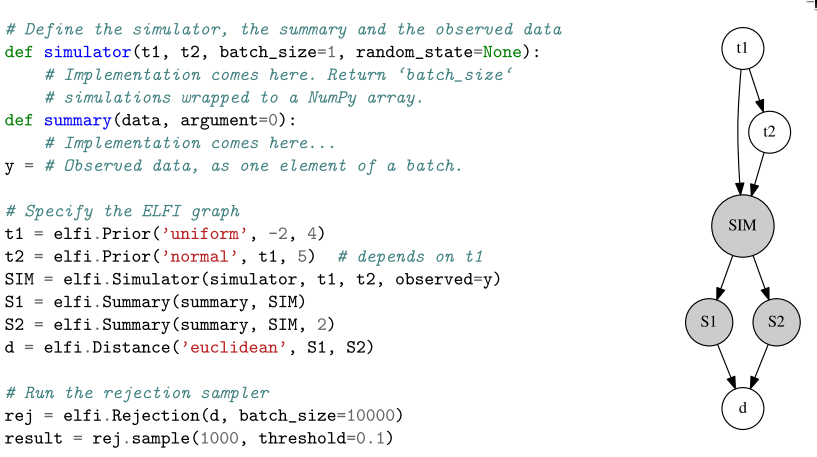
\includegraphics[width=0.8\textwidth]{./Thesis/images/chapter2/elfi.png}
    \end{center}
    \caption{Image taken from \cite{1708.00707}}
    \label{fig:elfi}
\end{figure}


\subsubsection{Inference Methods}
\label{sec:inference-methods}

The inference Methods implemented at the ELFI follow some common
guidelines;

\begin{itemize}
\item the initial argument should is the output node of the model. It
  is followed by the rest hyper-parameters of the method.
\item each inference method provides a central sampling
  functionality. In most cases it is named
  \pinline{<method_name>.sample()}.
\end{itemize}

The collection of likelihood-free inference methods implemented so far
contain the \textit{ABC Rejection Sampler}, the \textit{Sequential
  Monte Carlo ABC Sampler} and the \textit{Bayesian Optimisation for
  Likelihood-Free Inference (BOLFI)}. The latter has methodological
similarities to the ROMC method that we implement in the current work.

The Engine for Likelihood-Free Inference (ELFI) \autocite{1708.00707}
is a Python package dedicated to Likelihood-Free Inference (LFI). ELFI
models in a convenient manner all the fundamental components of a
probabilistic model such as priors, simulators, summaries and
distances. Furthermore, ELFI already supports some recently proposed
likelihood-free inference methods.

\subsubsection{Modelling}
\label{sec:modelling}

ELFI models the probabilistic model as a Directed Acyclic Graph (DAG);
it implements this functionality based on the package
\pinline{NetworkX}, which is designed for creating general purpose
graphs. Although not restricted to that, in most cases the structure
of a likelihood-free model follows the pattern presented in
figure~\ref{fig:elfi}; there are edges that connect the prior
distributions to the simulator, the simulator is connected to the
summary statistics that consequently are connected to the
distance. The distance is the output node. Samples can be obtained
from all nodes through sequential sampling. The nodes that are defined
as \pinline{elfi.Prior}\footnote{The \pinline{elfi.Prior} functionality
  is a wrapper around the \pinline{scipy.stats} package.} are automatically
considered as the parameters of interest and are the only nodes that,
apart from sampling, should also provide PDF evaluation. The function
passed as argument in the \pinline{elfi.Summary} node can be any valid
Python function. Finally, the observations should be passed in the
appropriate node through the argument \pinline{observed}.

\begin{figure}[!ht]
    \begin{center}
      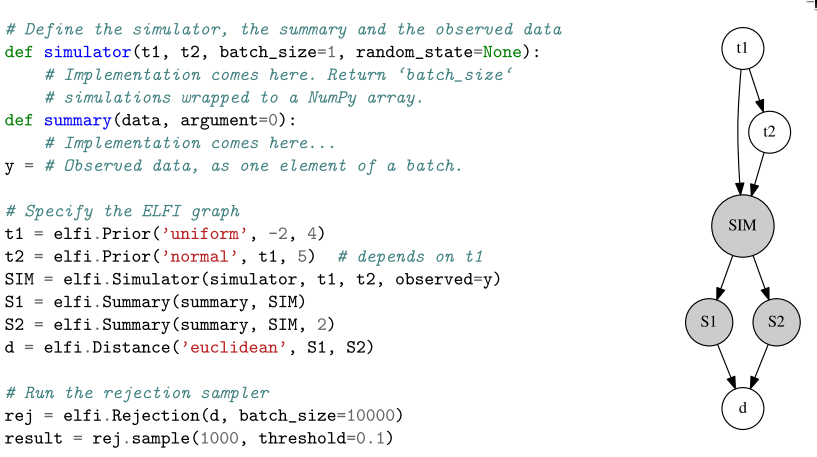
\includegraphics[width=0.8\textwidth]{./Thesis/images/chapter2/elfi.png}
    \end{center}
    \caption{Image taken from \cite{1708.00707}}
    \label{fig:elfi}
\end{figure}


\subsubsection{Inference Methods}
\label{sec:inference-methods}

The inference Methods implemented at the ELFI follow some common
guidelines;

\begin{itemize}
\item the initial argument should is the output node of the model. It
  is followed by the rest hyper-parameters of the method.
\item each inference method provides a central sampling
  functionality. In most cases it is named
  \pinline{<method_name>.sample()}.
\end{itemize}

The collection of likelihood-free inference methods implemented so far
contain the \textit{ABC Rejection Sampler}, the \textit{Sequential
  Monte Carlo ABC Sampler} and the \textit{Bayesian Optimisation for
  Likelihood-Free Inference (BOLFI)}. The latter has methodological
similarities to the ROMC method that we implement in the current work.


%%%%%%%%%%%%%%%%%%%%%%%%%%%%%%%%%%%%%%%% 
\clearpage
\section{Implementation}
In this chapter, we will analyse the details of the implementation of the ROMC inference method to the ELFI package. Sections \ref{subsec:general_design}, \ref{subsec:training}, \ref{subsec:inference}, \ref{subsec:utilities} provide an overview of the functionalities provided by our implementation. These three chapters analyse the implementation steps for training, performing the inference and evaluate the method from the point of view of the user. For illustration purposes, we will use a simple running example throughout the steps. In contrast, in the final section \ref{subsec:developers} we will delve into the internal details of the implementation in order to provide the information pieces for a possible extension of the method using user-defined methods as the internal building blocks.


\subsection{General Design}
\label{subsec:general_design}
% In figure \ref{fig:elfi-model} we present an overview of our
implementation; one could think of figure~\ref{fig:elfi-model} as a
depiction of the main class of our implementation, which is called
ROMC, while the entities inside the green and blue ellipses are the
main functions of the class. Following the common naming principles,
the methods starting with an underscore (green ellipses) represent
internal (private) functions and are not meant to be used by a user,
whereas the rest of the methods (blue ellipses) are the
functionalities used for performing the inference.As mentioned before,
the implementation favours extensibility; the building blocks that
compose the method have been designed in an isolated fashion so that a
practitioner may replace them without the method to collapse.

Figure \ref{fig:elfi-model} groups the ROMC implementation into the
training, the inference and the evaluation part, following the
arrangement used in the algorithmic presentation (section
\ref{subsec:romc-algorithmic}). The training part includes all the
steps until the computation of the proposal regions; sampling the
nuisance variables, defining the optimisation problems, solving them
and constructing the regions. The inference part comprises of
evaluating the unnormalised posterior (and the normalised one, in
low-dimensional cases), sampling and computing an
expectation. Moreover, the ROMC implementation provides some utilities
for inspecting the training process, such as plotting the histogram of
the distances
$d^*_i = g_i(\theta_i^*), \: \forall i \in \{1, \ldots, n_1
\}$ after solving the optimisation problems and visualising the
constructed bounding box\footnote{if the parametric space is up to
  $2D$}. Finally, there are implemented two functionalities for
evaluating the inference; (a) computing the Effective Sample Size
(ESS) of the obtained weighted samples and (b) measuring the
divergence of the approximate posterior from the ground-truth, if the
latter is available.\footnote{Normally, the ground-truth posterior is
  not available; that is the meaning of performing the inference!
  Though this functionality is useful in cases where the posterior can
  be computed numerically or with an alternative method (i.e.\ ABC
  Rejection Sampling) and we would like to measure the discrepancy
  between the two approximations.}


\subsubsection*{Simple 1D example}

For illustrating the implemented functionalities we choose as running
examples the following model, introduced by~\autocite{Ikonomov2019},

\begin{gather} \label{eq:1D_example}
  p(\theta) = \mathcal{U}(\theta;-2.5,2.5)\\
  p(y|\theta) = 
  \left\{
    \begin{array}{ll}
      \theta^4 + u & \mbox{if } \theta \in [-0.5, 0.5] \\
      |\theta| - c + u & \mbox{otherwise} 
    \end{array} \right.\\
  u \sim \mathcal{N}(0,1)
\end{gather}

\noindent
where $u \sim \mathcal{N}(0,1)$.

In the model \eqref{eq:1D_example}, the prior distribution is the
uniform in the range $[-2.5, 2.5]$ and the likelihood a Gaussian
distribution. There is only one observation $y_0 = 0$. The inference
in the particular example can be performed quite easily, without
icorporating a likelihood-free inference approach. Hence, we can
exploit it for validating the accuracy of our implementaion. The
ground-truth posterior, approximated computationally, is shown in
figure \ref{fig:example_gt}.

\begin{figure}[h]
    \begin{center}
      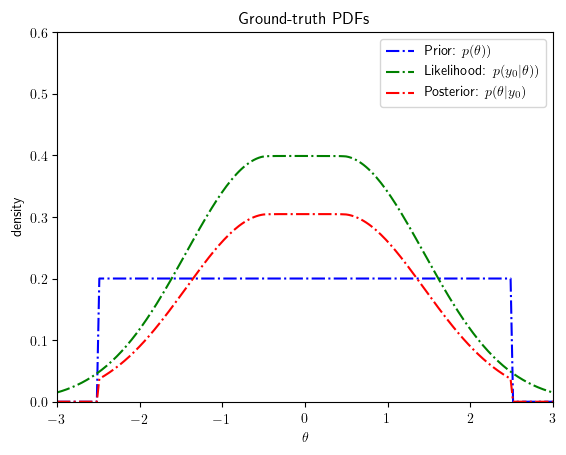
\includegraphics[width=0.5\textwidth]{./Thesis/images/chapter3/example_gt.png}
    \end{center}
  \caption{Ground-truth posterior distribution for our simple 1D example}
  \label{fig:example_gt}
\end{figure}

\subsubsection*{ELFI code for modelling the example}

In the following code snippet, we model the example as an
\textit{ELFI.Model} and we initialise the ROMC inference method. We
observe that the initialisation of the ROMC inference method is quite
intuitive; we just pass the final (distance) node of the simulator as
argument, as in all $\textit{ELFI}$ inference methods. The argument
\pinline{bounds}, although typically optional, is important for many
functionalities (e.g. approximating the partition function, set the bounds of the Bayesian optimisation etc.) so it is highly recommended to be passed.

\begin{pythoncode}
  import elfi
  import scipy.stats as ss
  import numpy as np
  
  def simulator(t1, batch_size=1,random_state=None):
      if t1 < -0.5:
          y = ss.norm(loc=-t1-c, scale=1).rvs(random_state=random_state)
      elif t1 <= 0.5:
          y = ss.norm(loc=t1**4, scale=1).rvs(random_state=random_state)
      else:
          y = ss.norm(loc=t1-c, scale=1).rvs(random_state=random_state)
      return y

  # observation
  y = 0
      
  # Elfi graph    
  t1 = elfi.Prior('uniform', -2.5, 5)
  sim = elfi.Simulator(simulator, t1, observed=y)
  d = elfi.Distance('euclidean', sim)

  # Define ROMC inference method
  bounds = [(-2.5, 2.5)]
  romc = elfi.ROMC(d, bounds=bounds)
\end{pythoncode}


\begin{figure}[!ht]
    \begin{center}
      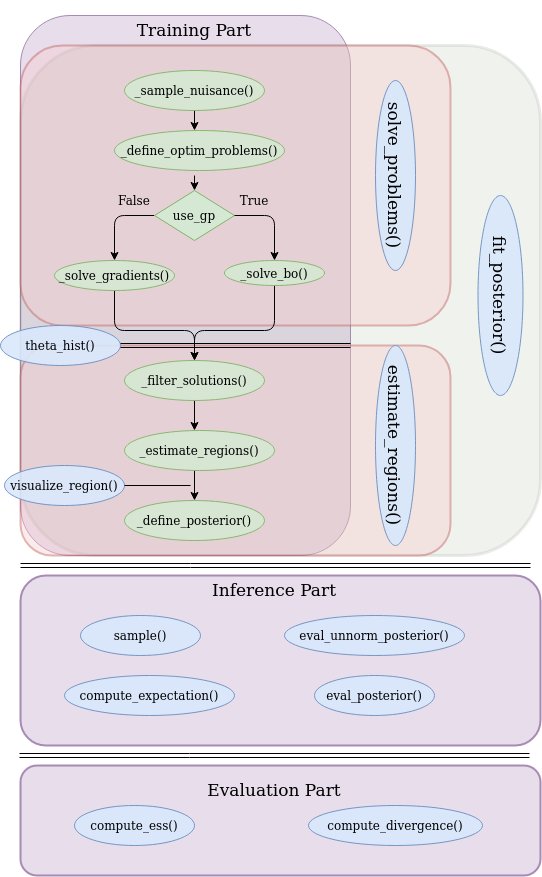
\includegraphics[width=0.8\textwidth]{./Thesis/graphs/ROMC.png}
    \end{center}
    \caption{Overview of the ROMC implementation. The training part
      follows a sequential pattern; the functions in the green
      ellipses must be called in a sequential fashion for completing
      the training part and define the posterior distribution. The
      functions in blue ellipses are the functionalities provided to
      the user.}
    \label{fig:elfi-model}
\end{figure}

  
In figure \ref{fig:elfi-model} we present an overview of our
implementation; one could think of figure~\ref{fig:elfi-model} as a
depiction of the main class of our implementation, which is called
ROMC, while the entities inside the green and blue ellipses are the
main functions of the class. Following the common naming principles,
the methods starting with an underscore (green ellipses) represent
internal (private) functions and are not meant to be used by a user,
whereas the rest of the methods (blue ellipses) are the
functionalities used for performing the inference.As mentioned before,
the implementation favours extensibility; the building blocks that
compose the method have been designed in an isolated fashion so that a
practitioner may replace them without the method to collapse.

Figure \ref{fig:elfi-model} groups the ROMC implementation into the
training, the inference and the evaluation part, following the
arrangement used in the algorithmic presentation (section
\ref{subsec:romc-algorithmic}). The training part includes all the
steps until the computation of the proposal regions; sampling the
nuisance variables, defining the optimisation problems, solving them
and constructing the regions. The inference part comprises of
evaluating the unnormalised posterior (and the normalised one, in
low-dimensional cases), sampling and computing an
expectation. Moreover, the ROMC implementation provides some utilities
for inspecting the training process, such as plotting the histogram of
the distances
$d^*_i = g_i(\theta_i^*), \: \forall i \in \{1, \ldots, n_1
\}$ after solving the optimisation problems and visualising the
constructed bounding box\footnote{if the parametric space is up to
  $2D$}. Finally, there are implemented two functionalities for
evaluating the inference; (a) computing the Effective Sample Size
(ESS) of the obtained weighted samples and (b) measuring the
divergence of the approximate posterior from the ground-truth, if the
latter is available.\footnote{Normally, the ground-truth posterior is
  not available; that is the meaning of performing the inference!
  Though this functionality is useful in cases where the posterior can
  be computed numerically or with an alternative method (i.e.\ ABC
  Rejection Sampling) and we would like to measure the discrepancy
  between the two approximations.}


\subsubsection*{Simple 1D example}

For illustrating the implemented functionalities we choose as running
examples the following model, introduced by~\autocite{Ikonomov2019},

\begin{gather} \label{eq:1D_example}
  p(\theta) = \mathcal{U}(\theta;-2.5,2.5)\\
  p(y|\theta) = 
  \left\{
    \begin{array}{ll}
      \theta^4 + u & \mbox{if } \theta \in [-0.5, 0.5] \\
      |\theta| - c + u & \mbox{otherwise} 
    \end{array} \right.\\
  u \sim \mathcal{N}(0,1)
\end{gather}

\noindent
where $u \sim \mathcal{N}(0,1)$.

In the model \eqref{eq:1D_example}, the prior distribution is the
uniform in the range $[-2.5, 2.5]$ and the likelihood a Gaussian
distribution. There is only one observation $y_0 = 0$. The inference
in the particular example can be performed quite easily, without
icorporating a likelihood-free inference approach. Hence, we can
exploit it for validating the accuracy of our implementaion. The
ground-truth posterior, approximated computationally, is shown in
figure \ref{fig:example_gt}.

\begin{figure}[h]
    \begin{center}
      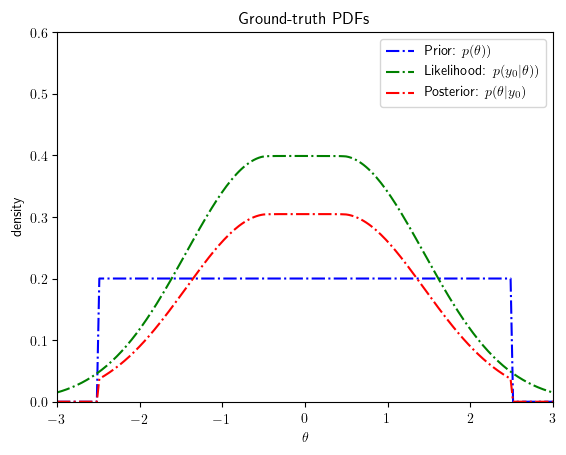
\includegraphics[width=0.5\textwidth]{./Thesis/images/chapter3/example_gt.png}
    \end{center}
  \caption{Ground-truth posterior distribution for our simple 1D example}
  \label{fig:example_gt}
\end{figure}

\subsubsection*{ELFI code for modelling the example}

In the following code snippet, we model the example as an
\textit{ELFI.Model} and we initialise the ROMC inference method. We
observe that the initialisation of the ROMC inference method is quite
intuitive; we just pass the final (distance) node of the simulator as
argument, as in all $\textit{ELFI}$ inference methods. The argument
\pinline{bounds}, although typically optional, is important for many
functionalities (e.g. approximating the partition function, set the bounds of the Bayesian optimisation etc.) so it is highly recommended to be passed.

\begin{pythoncode}
  import elfi
  import scipy.stats as ss
  import numpy as np
  
  def simulator(t1, batch_size=1,random_state=None):
      if t1 < -0.5:
          y = ss.norm(loc=-t1-c, scale=1).rvs(random_state=random_state)
      elif t1 <= 0.5:
          y = ss.norm(loc=t1**4, scale=1).rvs(random_state=random_state)
      else:
          y = ss.norm(loc=t1-c, scale=1).rvs(random_state=random_state)
      return y

  # observation
  y = 0
      
  # Elfi graph    
  t1 = elfi.Prior('uniform', -2.5, 5)
  sim = elfi.Simulator(simulator, t1, observed=y)
  d = elfi.Distance('euclidean', sim)

  # Define ROMC inference method
  bounds = [(-2.5, 2.5)]
  romc = elfi.ROMC(d, bounds=bounds)
\end{pythoncode}


\begin{figure}[!ht]
    \begin{center}
      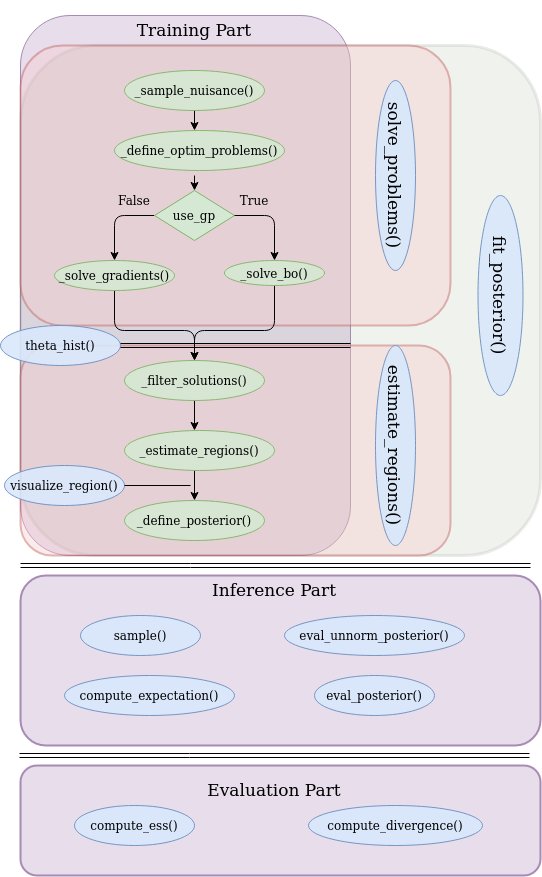
\includegraphics[width=0.8\textwidth]{./Thesis/graphs/ROMC.png}
    \end{center}
    \caption{Overview of the ROMC implementation. The training part
      follows a sequential pattern; the functions in the green
      ellipses must be called in a sequential fashion for completing
      the training part and define the posterior distribution. The
      functions in blue ellipses are the functionalities provided to
      the user.}
    \label{fig:elfi-model}
\end{figure}

  
lllllllllllllllllllllllllllllllallll
\subsection{Training}
\label{subsec:training}
The training part contains the 6 following functionalities:

\begin{itemize}
\item \mintinline{python}{romc.solve_problems(n1, use_bo=False, optimizer_args=None, seed=None)}
\item \mintinline{python}{romc.estimate_regions(eps_filter,}
  
      \mintinline{python}{                      use_surrogate=None, region_args=None,}
  
      \mintinline{python}{                      fit_models=False, fit_models_args=None,}
  
      \mintinline{python}{                      eps_region=None, eps_cutoff=None)}
      
    \item \mintinline{python}{romc.fit_posterior(n1, eps_filter, use_bo=False, optimizer_args=None,}
  
          \mintinline{python}{                   seed=None, use_surrogate=None, region_args=None,}
  
          \mintinline{python}{                   fit_models=False, fit_models_args=None,}
  
          \mintinline{python}{                   eps_region=None, eps_cutoff=None)}

\item \mintinline{python}{romc.distance_hist(savefig=False, **kwargs)}
\item \mintinline{python}{romc.visualize_region(i, savefig=False)}
\item \mintinline{python}{romc.compute_eps(quantile)}
\end{itemize}


\subsubsection*{Function (i): Define and solve the optimisation problems}

\pinline{romc.solve_problems(n1, use_bo=False, optimizer_args=None, seed=None)}
\vspace{5mm}

\noindent
This routine is responsible for (a) drawing the nuisance variables,
(b) define the optimisation problems and (c) solve them using either a
gradient-based optimiser or Bayesian optimisation. The aforementioned
tasks are done in a sequential fashion, as show in
figure~\ref{fig:elfi-model}. The defininition of the optimisation
problems is performed by drawing $n_1$ integer numbers from a discrete
uniform distribution $u_i \sim \mathcal{U}\{1, 2^{32}-1\}$. Each
integer $u_i$ is the seed used in ELFI's random simulator. Hence from
an algorithmic point-of-view drawing the state of all random
variables $\vb_i$ as described in the previous chapter, traces back to
just setting the seed that initialises the state of the pseudo-random
generator, before asking a sample from the simulator.

Finally, passing an integer number as the argument \pinline{seed}
absorbs all the randomness of the optimistation part (e.g.\ drawing
initial points for the optimisation procedure), making the whole
process reproducible.

Setting the argument \pinline{use_bo=True}, chooses the Bayesian
Optimisation scheme for obtaining $\theta_i^*$. In this case the
function $g_i(\thetab) = d(M_d(\thetab,\vb=\vb_i))$ which by default
is evaluated using the simulator, is replaced by a Gaussian Proccess
surrogate model $\hat{d}$, which is used in all next steps.

\subsubsection*{Function (ii): Construct bounding boxes and fit local surrogate models}

\mintinline{python}{romc.estimate_regions(eps_filter,}
  
      \mintinline{python}{                      use_surrogate=None, region_args=None,}
  
      \mintinline{python}{                      fit_models=False, fit_models_args=None,}
  
      \mintinline{python}{                      eps_region=None, eps_cutoff=None)}
\vspace{5mm}

\noindent
This function return the appropriate distance value $d_{i=\kappa}^*$
where $\kappa = \lfloor \frac{quantile}{n} \rfloor$ from the
collection $\{ d_i^* \} \forall i = \{1, \ldots, n\}$ where $n$ is the
number of accepted solutions. It can be used to automate the selection
of the threshold $\epsilon$, e.g.\
\pinline{eps=romc.compute_eps(quantile=0.9)}.

\subsubsection*{Function (iii): Perform all training steps in a single call}


\mintinline{python}{romc.fit_posterior(n1, eps_filter, use_bo=False, optimizer_args=None,}
  
          \mintinline{python}{                   seed=None, use_surrogate=None, region_args=None,}
  
          \mintinline{python}{                   fit_models=False, fit_models_args=None,}
  
          \mintinline{python}{                   eps_region=None, eps_cutoff=None)}

\vspace{5mm}
\noindent

This function constructs the bounding boxes around the optimal points
$\thetab_i^* : i = 1, 2, \ldots, n_1$ following the
Algorithm~\ref{alg:region_construction}. The Hessian matrix is
approximated based on the Jacobian $\hess_i = \jac_i^T \jac_i$. The
eigenvectores are computed using the function
\pinline{numpy.linalg.eig()} that calls, under the hood, the
\pinline{_geev LAPACK}. A check is performed so that the matrix
$\hess_i$ is not singular; if this is the case, the eigenvectors are
set to be the vectors of the orthonormal basis. Afterwards, the limits
are obtained by repeteadly querying the distance function
($g_i(\thetab)$ or $\hat{d}(\thetab)$) along the search directions. In
section \ref{subsec:developers}, we provide some details regarding the
way the bounding box is defined as a class and sampling is performed
on it.


\subsubsection*{Function (iv): Plot the histogramm of the optimal points}

\pinline{romc.distance_hist(**kwargs)}
\vspace{5mm}
\noindent

This function merges all steps for constructing the bounding box into
a single command. If the user doesn't want to manually inspect the
histogram of the distances before deciding where to set the threshold
$\epsilon$, he may call \pinline{romc.fit_posterior()} and the whole
training part will be done end-to-end. There are two alternatives for
setting the threshold $\epsilon$; the first is to set to a specific
value blindly and the second is to set at as a specific quantile of
the histogram of distances. In the second scenario the
\pinline{quantile} argument must be set to a floating number in the
range $[0,1]$ and \pinline{eps='auto'}.

\subsubsection*{Function (v): Plot the acceptance region of the objective functions}

\pinline{romc.visualize_region(i)}
\vspace{5mm}
\noindent

This function can serve as an intermediate step of manual inspection,
for helping the user choose which threshold $\epsilon$ to use. It
plots a histogram of the distances at the optimal point
$g_i(\thetab_i^*) : \{i = 1, 2, \ldots, n_1\}$ or
$d_i^*$ in case \pinline{use_bo=True}. The function accepts all
keyword arguments and forwards them to the underlying
\pinline{matplotlib.hist()} function; in this way the user may
customize some properties of the histogram, such as the number of bins
or the range of values.

\subsubsection*{Function (vi): Compute $\epsilon$ automatically based on the distribution of $d^*$}

\pinline{romc.compute_eps(quantile)}
\vspace{5mm}
\noindent

It can be used as an inspection utility for cases where the parametric
space is up to two dimensional. The argument $\pinline{i}$ is the
index of the corresponding optimization problem i.e.\ $i<n_1$.

\subsubsection*{Example}

Here we will illustrate the aforementioned functionalities using the
simple 1D example we set up in the previous chapter. The following
code snippet performs the training part at ELFI.

\begin{pythoncode}
  n1 = 500
  seed = 21
  eps = .75
  use_bo = False # True, if using Bayesian optimisation

  # Training set-by-step
  romc.solve_problems(n1=n1, seed=seed, use_bo=use_bo)
  romc.theta_hist(bins=100)
  romc.estimate_regions(eps=eps)
  romc.visualize_region(i=1)

  # Equivalent one-line command
  # romc.fit_posterior(n1=n1, eps=eps, use_bo=use_bo, seed=seed)
\end{pythoncode}

As stated before, switching to the Bayesian optimisation scheme needs
nothing more the setting the argument \pinline{use_bo=True}; all the
following command remain unchanged. In figure
\ref{fig:example_training} we illustrate the distribution of the
distances obtained and the acceptance area of the first optimisation
problem. We observe that most optimal points produce almost zero
distance.

\begin{figure}[h]
    \begin{center}
      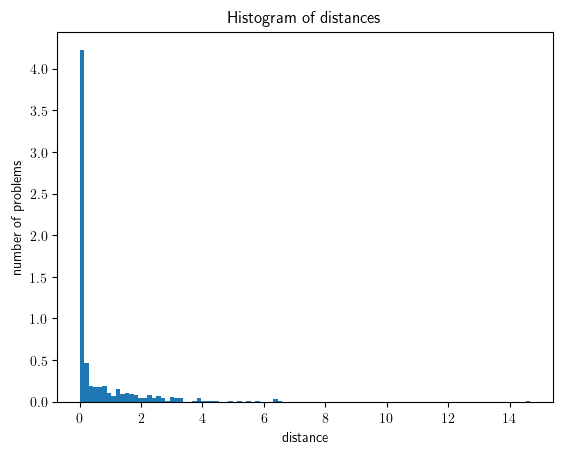
\includegraphics[width=0.48\textwidth]{./Thesis/images/chapter3/example_theta_dist.png}
      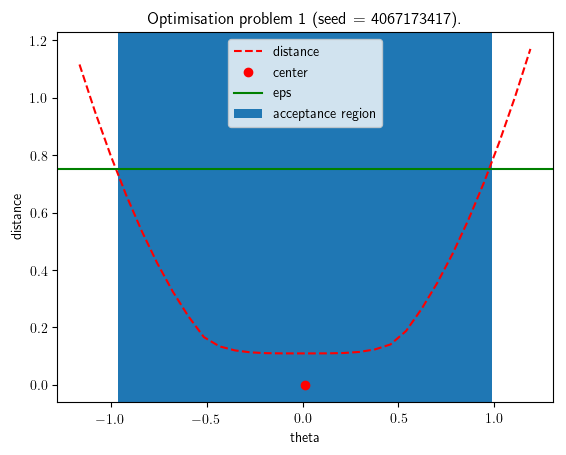
\includegraphics[width=0.48\textwidth]{./Thesis/images/chapter3/example_region.png}
    \end{center}
  \caption{Histogram of distances and visualisation of a specific region.}
  \label{fig:example_training}
\end{figure}


\subsection{Performing the Inference}
\label{subsec:inference}

\subsection{Utilities}
\label{subsec:utilities}

\subsection{Implementation details for developers}
\label{subsec:developers}

\clearpage
\section{Experiments}

\subsection{Another Example}

\subsection{Execution Time Experiments}

\section{Conclusions}

\subsection{Outcomes}

\subsection{Future Research Directions}
\clearpage

\printbibliography
\clearpage

\appendix
\section*{Appendices}
\addcontentsline{toc}{section}{Appendices}

\clearpage
\section{An Appendix}
\label{app:one}

Some stuff.
\clearpage

\section{Another Appendix}
\label{app:two}

Some other stuff.



\end{document}
